\chapter{\label{ch:polycubes2}Designing polycube assembly rules}

\minitoc

In the previous chapter, we used random input rules to explore the properties of the corresponding distributions of output polycube shapes. However, the reverse problem is just as significant; given a target shape, how do you find a rule that assembles it?

This chapter provides a method for systematically enumerating valid solutions and discovering minimal solutions for arbitrary shapes. Section~\ref{sec:SAT} describes how this is done, with the following sections providing examples of designed shapes and their assembly dynamics.

% Fully addressable is the easy solution.

A trivial solution for designing a polycube shape would be to use \emph{fully addressable assembly}: simply assign a unique species to each cube and a unique colour to each pair of adjacent patches. This is similar to the design principle underlying DNA bricks (Section~\ref{sec:dna_tiles_bricks}), where every brick tile is unique. However, as was seen in Chapter~\ref{ch:polycubes1}, many shapes have alternative solutions requiring widely different numbers of unique components. 

\begin{figure}[h]
    \centering
    \begin{overpic}[width=\textwidth]{figures/solve/adressable.eps}
        \put(-10,480){a)}
        \put(360,580){b)}

        \put(370, 350){\makebox(0,0){\rotatebox{90}{Number of colours (\(\widetilde{K}_c\))}}}
        \put(600,-30){Number of species (\(\widetilde{K}_s\))}
    \end{overpic}
    \vspace{1em}
    %\includesvg[width=\textwidth, inkscapelatex=false]{figures/solve/adressable.svg}
    \caption{\(2 \times 2\) square polyomino assembled with different levels of complexity. \textbf{a)} Schematic of the input shape, consisting of four connected tiles. \textbf{b)} The green region shows possible assembly solutions, from the \emph{minimal solution} using a single species and a single colour (bottom left), to the \emph{fully addressable solution} using four species and colours (top right). The red region lacks solutions. }
    \label{fig:addressable}
\end{figure}

Figure~\ref{fig:addressable} shows a square tetromino with a variety of inputs assembling it, from the minimal solution with just a single species and one colour, up to the fully addressable solution with four species and four colours (\(\widetilde{K}_s = \widetilde{K}_c = 4\)). The intermediate solutions are not necessarily deterministic in terms of which position gets which species, but they will always assemble into the same shape. Some solutions may also be able to form with only three bonds if the fourth patch pair has mismatched colours. However, such an assembly would be less stable than the assemblies shown in the figure. 

It can be argued that the solutions on the bottom row, where \(\widetilde{K}_c=1\), all technically use only one species since all species have identical patches. However, one could imagine an additional property, such as different functionalisation, motivating the distinction. The empty red region in Figure~\ref{fig:addressable}.b) shows combinations of \(\widetilde{K}_s\) and \(\widetilde{K}_c\) for which a solution is not possible. For example, if you use a single species, you cannot use more than one colour.



So, how do we find alternative and simpler input rules for a shape? Surely, there must exist a better method than sampling the space of all rules (as done in Chapter~\ref{ch:polycubes1})‽ This chapter presents an approach where \emph{satisfiability solving} is used to determine if a shape can be assembled from a given number of colours and species, thus automatically creating solution landscapes such as the one shown in Figure~\ref{fig:addressable}.
%A complementary approach substituting similar species is also described in Section~\ref{sec:substitution_solving}.


\section{Satisfiability solving}
\label{sec:SAT}

Building upon a published method for determining patchy particle interactions for unbounded structures \cite{romano2020designing}, it is possible to formulate and solve satisfiability problems that map onto assembly rules for the bounded polycubes.

In essence, we formulate a boolean expression that, if true, means it is possible to assemble a given polycube topology using a given number of colours and species. We can then use a satisfiability solver such as Glucose \cite{audemard2009glucose, imms-sat18} to check if that expression is indeed solvable and, if it is, extract an assembly rule from the solution.

\subsection{Boolean expressions}

The boolean expression is written in conjunctive normal form (CNF), where variables are composed into clauses using \emph{NOT} (\(\lnot\)) and \emph{OR} (\(\lor\)) operators and where the clauses are joined by \emph{AND} (\(\land\)) operators. As a simple example, see the expression below:

\[
    (\lnot x_{rain} \lor x_{umbrella} \lor  \lnot x_{walk}) \land
    (\lnot x_{rainbow} \lor x_{rain}) \land
    (\lnot x_{rainbow} \lor x_{sunny})
\]

The first clause is \({true}\) for all values except when \(x_{rain}={true}\), \(x_{umbrella}={false}\) and \(x_{walk}=true\); so the solution of taking a walk in the rain without an umbrella is forbidden. This could also be written as an \emph{implication}: \(x_{rain} \land x_{walk} \implies x_{umbrella}\).

The following two clauses in the example above are the CNF form of another implication: \(x_{rainbow} \implies  x_{rain} \land x_{sunshine}\), stating that a rainbow implies that we have both rain and sunshine (we cannot have a rainbow without rain or without sunshine). The full expression is satisfiable, for example, if we set \(x_{sun}=true\), \(x_{rain}=false\), \(x_{walk}=false\), \(x_{umbrella}=false\), and \(x_{rainbow}=false\); ignoring the walk in the sunshine and remaining inside to work.

\subsection{Polycube formulation}

For the polycube problem, we introduce the following variables:
\begin{description}
    \item[\(x_{l,p,o}^{A}\)] (patch \(p\) at position \(l\) has orientation \(o\))
    \item[\(x_{c_i,c_j}^{B}\)] (colour \(c_i\) is compatible with colour \(c_j\))
    \item[\(x_{s,p,c}^{C}\)] (patch \(p\) on species \(s\) has colour \(c\))
    \item[\(x_{p_1,o_1,p_2,o_2}^{D}\)] (patch \(p_1\) with orientation \(o_1\) binds to patch \(p_2\) with orientation \(o_2\))
    \item[\(x_{l,p,c}^{F}\)] (patch \(p\) at position \(l\) has colour \(c\))
    \item[\(x_{s,p,o}^{O}\)] (patch \(p\) on species \(s\) has orientation \(o\))
    \item[\(x_{l,s,r}^{P}\)] (position \(l\) is occupied by species \(s\) rotated by \(r\))] 
\end{description}

We then formulate clauses to constrain the problem, seen in Table~\ref{tab:sat_clauses}. Clauses (i)-(vii) are the same as in \cite{romano2020designing} while the remaining are added, together with variables \(x^D\), \(x^A\) and \(x^O\) above, to include \emph{torsional restrictions}, meaning that patches need to bind at a compatible orientation (compared to being allowed to rotate freely).

\begin{table}[h!]
    \centering
    \begin{tabular}{|c|l|l|p{5cm}|}
        \hline
        & Clause & Boolean expression & Description \\ 
        \hline
        \hline
        (i) & \(C^{B}_{c_i,c_j,c_k}\) & \(\neg x_{c_i,c_j}^{B} \lor \neg x_{c_i,c_k}^{B}\) & \small{Each colour is compatible with \textit{exactly one} colour.} \\ % Each colour is compatible with exactly one colour
        (ii) &  \(C^{C}_{s,p,c_k,c_l}\) & \(\neg x_{s, p, c_k}^{C} \lor \neg x_{s, p, c_l}^{C}\) & \small{Each patch has \textit{exactly one} colour.}  \\ % Each patch is assigned exactly one colour
        (iii) & \(C^{P}_{l, s_i, r_i, s_j, r_j}\)  & \(\neg x_{l,s_i,r_i}^{P} \lor \neg x_{l,s_j,r_j}^{P} \) & \small{Each lattice position contains a single species with an assigned rotation.} \\ % Each lattice position is occupied by a single species with one assigned rotation
        (iv) & \(C^{BF}_{l_i,p_i,c_i,l_j,p_j,c_j}\) & \(\left(x_{l_i,p_i,c_i}^{F} \land x_{l_j,p_j,c_j}^{F} \right) \Rightarrow x_{c_i,c_j}^{B}\) & \small{Adjacent patches in the lattice must have compatible colours.}  \\ % Colours of patches that interact in the target lattice must be compatible
        (v) & \(C^{rotC}_{l,s,r,p,c}\) & \(x_{l,s,r}^{P} \Rightarrow \left(x_{l,p,c}^{F} \Leftrightarrow x_{s, \phi_r(p), c}^{C}\right)\) & \small{Patches at a lattice position are coloured according to the (rotated) occupying species (see Table~\ref{tab:cubeRotations})} \\ % The patches at a lattice position is set to have the patch colours of the rotated occupying species.
        (vi) & \(C^{all s}_{s}\)  & \(\bigvee_{\forall l, r} x_{l,s,r}^{P}\) & \small{All species are required in the solution.} \\ % All \widetilde{K}_s species are used for the lattice assembly
        (vii) & \(C^{all c}_{c}\)  & \(\bigvee_{\forall s, p} x_{s,p,c}^{C}\) & \small{All patch colours are required in the solution.}  \\ % All \widetilde{K}_c patch colours are used in the solution
        (viii) &  \(C^{O}_{s,p,o_k,o_l}\) & \(\neg x_{s, p, o_k}^{O} \lor \neg x_{s, p, o_l}^{O}\) & \small{Each patch is assigned \textit{exactly one} orientation.} \\ % Each patch is assigned exactly one orientation
        (ix) & \(C^{DA}_{l_i,p_i,c_i,l_j,p_j,c_j}\) & \(\left(x_{l_i,p_i,c_i}^{A} \land x_{l_j,p_j,c_j}^{A} \right) \Rightarrow x_{p_i,c_i,p_j,c_j}^{D}\) & \small{Adjacent patches in the target lattice must have the same orientation.} \\ % Orientation of patches that interact in the target lattice must be compatible
        (x) & \(C^{rotO}_{l,s,r,p,o}\) & \(x_{l,s,r}^{P} \Rightarrow \left(x_{l,p,o}^{A} \Leftrightarrow x_{s, \phi_r(p), o}^{O}\right)\) & \small{Patches at a lattice position are oriented according to the (rotated) occupying species.} \\ % The patches at a lattice position is set to have the orientations of the rotated occupying species.
        \hline
    \end{tabular}
    \caption{Polycube SAT clauses and their descriptions.}
    \label{tab:sat_clauses}
    \end{table}

Note that for 3D polycubes, there are six patches per species instead of the four seen in the 2D polyominoes. Compared to the 4 square rotations defined for 2D \cite{romano2020designing}, this also introduces 27 possible cube rotations, seen in Table~\ref{tab:cubeRotations}, where $\phi_r(p)$ corresponds to the patch number that will overlap with original patch number $p$ at rotation $r$

\begin{table}[h]
    \centering
    \caption{List of all possible rotations to superpose a cube onto itself. The value at index \(p\) in a mapping corresponds to the patch number that is now positioned where patch number \(p\) was before the rotation.}
    \begin{tabular}{|r|r|}
    \hline
    Rotation \(r\) & Mapping \(\phi_r\) \\
    \hline
    \hline
    0 & (0,  1,  2,  3,  4,  5) \\
    1 & (0,  1,  3,  2,  5,  4) \\
    2 & (0,  1,  4,  5,  3,  2) \\
    3 & (0,  1,  5,  4,  2,  3) \\
    4 & (1,  0,  2,  3,  5,  4) \\
    5 & (1,  0,  3,  2,  4,  5) \\
    6 & (1,  0,  4,  5,  2,  3) \\
    7 & (1,  0,  5,  4,  3,  2) \\
    8 & (2,  3,  0,  1,  5,  4) \\
    9 & (2,  3,  1,  0,  4,  5) \\
    10 & (2,  3,  4,  5,  0,  1) \\
    11 & (2,  3,  5,  4,  1,  0) \\
    12 & (3,  2,  0,  1,  4,  5) \\
    13 & (3,  2,  1,  0,  5,  4) \\
    14 & (3,  2,  4,  5,  1,  0) \\
    15 & (3,  2,  5,  4,  0,  1) \\
    16 & (4,  5,  0,  1,  2,  3) \\
    17 & (4,  5,  1,  0,  3,  2) \\
    18 & (4,  5,  2,  3,  1,  0) \\
    19 & (4,  5,  3,  2,  0,  1) \\
    20 & (5,  4,  0,  1,  3,  2) \\
    21 & (5,  4,  1,  0,  2,  3) \\
    22 & (5,  4,  2,  3,  0,  1) \\
    23 & (5,  4,  3,  2,  1,  0) \\
    \hline
    \end{tabular}
    \label{tab:cubeRotations}
\end{table}

\subsection{On the importance of torsional interactions}

It is possible to use the solver without any constraints on the patch orientations (as it was done in \cite{romano2020designing}). However, if we wanted to use the stochastic assembler from Chapter~\ref{ch:polycubes1}, orientations would have to be assigned randomly, resulting in a combinatoric explosion of additional assembly paths.

More importantly, the assembly should benefit from torsional patch interaction (for 2D polyominoes, this corresponds to the requirement that tiles can be rotated in the plane but not flipped). Figure~\ref{fig:torsion} shows two versions of a simple rule, the only difference being the orientation of a single patch. While co--operative binding might, in such a case, benefit the desired square assembly, the self--limiting ability would be significantly improved if the patches were torsionally rigid.

\begin{figure}[h]
    \centering
    \begin{overpic}[width=\textwidth]{figures/torsion.png}
        \put(0,470){a)}
        \put(550,500){b)}
    \end{overpic}
    \caption{The consequences of a rotated patch. \textbf{a)} A minimal solution (one species and one colour) for a \(2 \times 2\) square. \textbf{b)} The same rule as a), except one patch on is rotated by \(\frac{\pi}{2}\).}
    \label{fig:torsion}
\end{figure}


\subsection{Bounded structures}
Besides the torsional patches, another important difference to \cite{romano2020designing} is that the method presented here allows for bounded structures. This is achieved by adding species of type \emph{empty} as a ``shell'' around the shape to ensure that empty patches remain unbound. Adding a clause \(x_{0,1}^{B}\) ensures that the colour 0 (on the shell) binds to colour 1 (on the boundary). 

\begin{figure}[h]
    \centering\includesvg[width=.5\textwidth, inkscapelatex=false]{figures/sat_boundary.svg}
    \caption{Bounded shape topology for satisfiability solving. Patches at the boundary of the shape (white) are constrained to only bind to ``empty''. 3D shapes are specified the same way, but with six patches per species.}
    \label{fig:sat_boundary}
\end{figure}


We then add clauses \(x_{l,p,1}^{F}\) to constrain every boundary patch \(p\) at lattice position \(l\) to have the colour \(1\) and thereby not bind anything else. For example, in Figure~\ref{fig:sat_boundary}, where these boundary patches are seen coloured white (and bordering an empty square), we get the following 12 clauses:

\begin{equation}
    \begin{aligned}
        &x_{0,0,1}^{F} \land x_{0,1,1}^{F} \land x_{0,3,1}^{F} \land \\
        &x_{1,0,1}^{F} \land x_{1,2,1}^{F} \land x_{1,3,1}^{F} \land \\
        &x_{3,0,1}^{F} \land x_{3,1,1}^{F} \land x_{3,2,1}^{F} \land \\
        &x_{4,1,1}^{F} \land x_{4,2,1}^{F} \land x_{4,3,1}^{F}
    \end{aligned}
\end{equation}

The topology of the shape is enforced by clause (iv), \(\left(\lnot x_{l_1, p_1, c_1}^{F} \lor \lnot x_{l_2, p_2, c_2}^{F} \lor x_{c_1, c_2}^{B}\right)\) in CNF, making sure that if patch \(p_1\) on lattice position \(l_1\) binds to \(p_2\) on lattice position \(l_2\), their colours are compatible. Similarly, clause (ix) ensures that the patches have the same orientation.

% Figure of topology graph?

\subsection{Interaction matrix}
Compared to \cite{romano2020designing}, the polycube interaction matrix is by default fixed. Thus, the \(x_{c_i,c_j}^{B}\) variable has fixed values and we only need to extract the values of \(x_{l,p,c}^{F}\) and \(x_{s,p,o}^{O}\) to construct the assembly rule. Note, however, that it is still possible to re--enable a variable interaction matrix, something which could prove useful for some shapes where, for example, self--complementary patches would result in a lower complexity.

Compared to the interaction matrix convention used in Chapter~\ref{ch:polycubes1}, where each colour \(c\) binds to \(-c\), the colour values in the SAT solver remain unsigned and instead pair each even colour \(c\) to the odd \(c+1\). The colour pairs are mapped back to the polycube convention when obtaining the solution.

\subsection{Assembly determinism}
Even if the SAT solver determines that a solution exists, it is still possible that the rule we get can also assemble into other shapes. Recall, once more, the ``giraffe duck'' shape from Figure~\ref{fig:UND}.b). If we solved for the shape with two neck cubes, the non--deterministic rule shown would be a perfectly valid solution according to the SAT solver, even though it can also produce giraffe ducks with any other neck length.

Because of this, we once again use the stochastic assembler to verify that the rule assembles into the correct shape every time. Each potential rule is evaluated a large number of times (by default \(100\)), calculating an assembly ratio. If the ratio is \(1\), the rule is considered bounded and deterministic and, as such, a valid solution.


\subsection{Finding the minimal assembly rule}

By iteratively ruling out lower values of \(\widetilde{K}_s\) and \(\widetilde{K}_c\), a minimal solution can be found, as detailed in Figure~\ref{fig:sat_alg}. It is also possible to generate and compare alternative solutions of varying complexity. While forbidding an undefined solution and retrying could in principle, continue until the computer runs out of memory (or the solution is disproven or valid), the results presented below used a limit of 100 retries before moving on. It is thus possible, albeit unlikely, that the actual minimal solutions were missed, but the solutions found can at least be claimed to be minimised. Instead of interatively forbidding solutions, it is possible to use a solver like Relsat\footnote{Found at \url{https://code.google.com/archive/p/relsat}} to obtain multiple solutions at once, but this also has no guarantee of finding all solutions with the memory available.

The exploration of the solution landscape can be done in parallel, with each combination of \(\widetilde{K}_s\) and \(\widetilde{K}_c\) explored concurrently.

\begin{figure}
    \centering
    \resizebox{\textwidth}{!}{% Graphic for TeX using PGF
% Title: /home/joakim/Documents/polycube/SAT_flow.dia
% Creator: Dia v0.97+git
% CreationDate: Thu May 27 10:43:08 2021
% For: joakim
% \usepackage{tikz}
% The following commands are not supported in PSTricks at present
% We define them conditionally, so when they are implemented,
% this pgf file will use them.
\ifx\du\undefined
  \newlength{\du}
\fi
\setlength{\du}{15\unitlength}
\begin{tikzpicture}[even odd rule]
\pgftransformxscale{1.000000}
\pgftransformyscale{-1.000000}
\definecolor{dialinecolor}{rgb}{0.000000, 0.000000, 0.000000}
\pgfsetstrokecolor{dialinecolor}
\pgfsetstrokeopacity{1.000000}
\definecolor{diafillcolor}{rgb}{1.000000, 1.000000, 1.000000}
\pgfsetfillcolor{diafillcolor}
\pgfsetfillopacity{1.000000}
\pgfsetlinewidth{0.100000\du}
\pgfsetdash{}{0pt}
\pgfsetmiterjoin
{\pgfsetcornersarced{\pgfpoint{0.000000\du}{0.000000\du}}\definecolor{diafillcolor}{rgb}{1.000000, 1.000000, 1.000000}
\pgfsetfillcolor{diafillcolor}
\pgfsetfillopacity{1.000000}
\fill (13.087793\du,24.536630\du)--(13.087793\du,26.436630\du)--(19.140293\du,26.436630\du)--(19.140293\du,24.536630\du)--cycle;
}{\pgfsetcornersarced{\pgfpoint{0.000000\du}{0.000000\du}}\definecolor{dialinecolor}{rgb}{0.000000, 0.000000, 0.000000}
\pgfsetstrokecolor{dialinecolor}
\pgfsetstrokeopacity{1.000000}
\draw (13.087793\du,24.536630\du)--(13.087793\du,26.436630\du)--(19.140293\du,26.436630\du)--(19.140293\du,24.536630\du)--cycle;
}% setfont left to latex
\definecolor{dialinecolor}{rgb}{0.000000, 0.000000, 0.000000}
\pgfsetstrokecolor{dialinecolor}
\pgfsetstrokeopacity{1.000000}
\definecolor{diafillcolor}{rgb}{0.000000, 0.000000, 0.000000}
\pgfsetfillcolor{diafillcolor}
\pgfsetfillopacity{1.000000}
\node[anchor=base,inner sep=0pt, outer sep=0pt,color=dialinecolor] at (16.114043\du,25.681630\du){Try \(N_c\) and \(N_t\)};
% setfont left to latex
\definecolor{dialinecolor}{rgb}{0.000000, 0.000000, 0.000000}
\pgfsetstrokecolor{dialinecolor}
\pgfsetstrokeopacity{1.000000}
\definecolor{diafillcolor}{rgb}{0.000000, 0.000000, 0.000000}
\pgfsetfillcolor{diafillcolor}
\pgfsetfillopacity{1.000000}
\node[anchor=base west,inner sep=0pt,outer sep=0pt,color=dialinecolor] at (27.290293\du,24.956775\du){Yes};
% setfont left to latex
\definecolor{dialinecolor}{rgb}{0.000000, 0.000000, 0.000000}
\pgfsetstrokecolor{dialinecolor}
\pgfsetstrokeopacity{1.000000}
\definecolor{diafillcolor}{rgb}{0.000000, 0.000000, 0.000000}
\pgfsetfillcolor{diafillcolor}
\pgfsetfillopacity{1.000000}
\node[anchor=base west,inner sep=0pt,outer sep=0pt,color=dialinecolor] at (24.240293\du,28.331775\du){No};
\pgfsetlinewidth{0.100000\du}
\pgfsetdash{}{0pt}
\pgfsetmiterjoin
{\pgfsetcornersarced{\pgfpoint{0.000000\du}{0.000000\du}}\definecolor{diafillcolor}{rgb}{1.000000, 1.000000, 1.000000}
\pgfsetfillcolor{diafillcolor}
\pgfsetfillopacity{1.000000}
\fill (39.101543\du,24.536630\du)--(39.101543\du,26.436630\du)--(42.064043\du,26.436630\du)--(42.064043\du,24.536630\du)--cycle;
}{\pgfsetcornersarced{\pgfpoint{0.000000\du}{0.000000\du}}\definecolor{dialinecolor}{rgb}{0.000000, 0.000000, 0.000000}
\pgfsetstrokecolor{dialinecolor}
\pgfsetstrokeopacity{1.000000}
\draw (39.101543\du,24.536630\du)--(39.101543\du,26.436630\du)--(42.064043\du,26.436630\du)--(42.064043\du,24.536630\du)--cycle;
}% setfont left to latex
\definecolor{dialinecolor}{rgb}{0.000000, 0.000000, 0.000000}
\pgfsetstrokecolor{dialinecolor}
\pgfsetstrokeopacity{1.000000}
\definecolor{diafillcolor}{rgb}{0.000000, 0.000000, 0.000000}
\pgfsetfillcolor{diafillcolor}
\pgfsetfillopacity{1.000000}
\node[anchor=base,inner sep=0pt, outer sep=0pt,color=dialinecolor] at (40.582793\du,25.681630\du){Done};
% setfont left to latex
\definecolor{dialinecolor}{rgb}{0.000000, 0.000000, 0.000000}
\pgfsetstrokecolor{dialinecolor}
\pgfsetstrokeopacity{1.000000}
\definecolor{diafillcolor}{rgb}{0.000000, 0.000000, 0.000000}
\pgfsetfillcolor{diafillcolor}
\pgfsetfillopacity{1.000000}
\node[anchor=base west,inner sep=0pt,outer sep=0pt,color=dialinecolor] at (37.640293\du,24.756775\du){Yes};
% setfont left to latex
\definecolor{dialinecolor}{rgb}{0.000000, 0.000000, 0.000000}
\pgfsetstrokecolor{dialinecolor}
\pgfsetstrokeopacity{1.000000}
\definecolor{diafillcolor}{rgb}{0.000000, 0.000000, 0.000000}
\pgfsetfillcolor{diafillcolor}
\pgfsetfillopacity{1.000000}
\node[anchor=base west,inner sep=0pt,outer sep=0pt,color=dialinecolor] at (33.890293\du,29.156775\du){No};
\pgfsetlinewidth{0.100000\du}
\pgfsetdash{}{0pt}
\pgfsetmiterjoin
\definecolor{diafillcolor}{rgb}{1.000000, 1.000000, 1.000000}
\pgfsetfillcolor{diafillcolor}
\pgfsetfillopacity{1.000000}
\fill (23.943082\du,23.300000\du)--(27.486164\du,25.486630\du)--(23.943082\du,27.673261\du)--(20.400000\du,25.486630\du)--cycle;
\definecolor{dialinecolor}{rgb}{0.000000, 0.000000, 0.000000}
\pgfsetstrokecolor{dialinecolor}
\pgfsetstrokeopacity{1.000000}
\draw (23.943082\du,23.300000\du)--(27.486164\du,25.486630\du)--(23.943082\du,27.673261\du)--(20.400000\du,25.486630\du)--cycle;
% setfont left to latex
\definecolor{dialinecolor}{rgb}{0.000000, 0.000000, 0.000000}
\pgfsetstrokecolor{dialinecolor}
\pgfsetstrokeopacity{1.000000}
\definecolor{diafillcolor}{rgb}{0.000000, 0.000000, 0.000000}
\pgfsetfillcolor{diafillcolor}
\pgfsetfillopacity{1.000000}
\node[anchor=base,inner sep=0pt, outer sep=0pt,color=dialinecolor] at (23.943082\du,25.681630\du){Satisfiable?};
\pgfsetlinewidth{0.100000\du}
\pgfsetdash{}{0pt}
\pgfsetmiterjoin
\definecolor{diafillcolor}{rgb}{1.000000, 1.000000, 1.000000}
\pgfsetfillcolor{diafillcolor}
\pgfsetfillopacity{1.000000}
\fill (33.444978\du,22.430375\du)--(37.941584\du,25.486630\du)--(33.444978\du,28.542886\du)--(28.948372\du,25.486630\du)--cycle;
\definecolor{dialinecolor}{rgb}{0.000000, 0.000000, 0.000000}
\pgfsetstrokecolor{dialinecolor}
\pgfsetstrokeopacity{1.000000}
\draw (33.444978\du,22.430375\du)--(37.941584\du,25.486630\du)--(33.444978\du,28.542886\du)--(28.948372\du,25.486630\du)--cycle;
% setfont left to latex
\definecolor{dialinecolor}{rgb}{0.000000, 0.000000, 0.000000}
\pgfsetstrokecolor{dialinecolor}
\pgfsetstrokeopacity{1.000000}
\definecolor{diafillcolor}{rgb}{0.000000, 0.000000, 0.000000}
\pgfsetfillcolor{diafillcolor}
\pgfsetfillopacity{1.000000}
\node[anchor=base,inner sep=0pt, outer sep=0pt,color=dialinecolor] at (33.444978\du,25.281630\du){Bounded \&};
% setfont left to latex
\definecolor{dialinecolor}{rgb}{0.000000, 0.000000, 0.000000}
\pgfsetstrokecolor{dialinecolor}
\pgfsetstrokeopacity{1.000000}
\definecolor{diafillcolor}{rgb}{0.000000, 0.000000, 0.000000}
\pgfsetfillcolor{diafillcolor}
\pgfsetfillopacity{1.000000}
\node[anchor=base,inner sep=0pt, outer sep=0pt,color=dialinecolor] at (33.444978\du,26.081630\du){Deterministic?};
\pgfsetlinewidth{0.100000\du}
\pgfsetdash{}{0pt}
\pgfsetmiterjoin
{\pgfsetcornersarced{\pgfpoint{0.000000\du}{0.000000\du}}\definecolor{diafillcolor}{rgb}{1.000000, 1.000000, 1.000000}
\pgfsetfillcolor{diafillcolor}
\pgfsetfillopacity{1.000000}
\fill (30.669978\du,29.741575\du)--(30.669978\du,32.441575\du)--(36.272478\du,32.441575\du)--(36.272478\du,29.741575\du)--cycle;
}{\pgfsetcornersarced{\pgfpoint{0.000000\du}{0.000000\du}}\definecolor{dialinecolor}{rgb}{0.000000, 0.000000, 0.000000}
\pgfsetstrokecolor{dialinecolor}
\pgfsetstrokeopacity{1.000000}
\draw (30.669978\du,29.741575\du)--(30.669978\du,32.441575\du)--(36.272478\du,32.441575\du)--(36.272478\du,29.741575\du)--cycle;
}% setfont left to latex
\definecolor{dialinecolor}{rgb}{0.000000, 0.000000, 0.000000}
\pgfsetstrokecolor{dialinecolor}
\pgfsetstrokeopacity{1.000000}
\definecolor{diafillcolor}{rgb}{0.000000, 0.000000, 0.000000}
\pgfsetfillcolor{diafillcolor}
\pgfsetfillopacity{1.000000}
\node[anchor=base,inner sep=0pt, outer sep=0pt,color=dialinecolor] at (33.471228\du,30.886575\du){Forbid current};
% setfont left to latex
\definecolor{dialinecolor}{rgb}{0.000000, 0.000000, 0.000000}
\pgfsetstrokecolor{dialinecolor}
\pgfsetstrokeopacity{1.000000}
\definecolor{diafillcolor}{rgb}{0.000000, 0.000000, 0.000000}
\pgfsetfillcolor{diafillcolor}
\pgfsetfillopacity{1.000000}
\node[anchor=base,inner sep=0pt, outer sep=0pt,color=dialinecolor] at (33.471228\du,31.686575\du){solution};
\pgfsetlinewidth{0.100000\du}
\pgfsetdash{}{0pt}
\pgfsetbuttcap
{
\definecolor{diafillcolor}{rgb}{0.000000, 0.000000, 0.000000}
\pgfsetfillcolor{diafillcolor}
\pgfsetfillopacity{1.000000}
% was here!!!
\pgfsetarrowsend{stealth}
\definecolor{dialinecolor}{rgb}{0.000000, 0.000000, 0.000000}
\pgfsetstrokecolor{dialinecolor}
\pgfsetstrokeopacity{1.000000}
\draw (19.188296\du,25.486630\du)--(20.400000\du,25.486630\du);
}
\pgfsetlinewidth{0.100000\du}
\pgfsetdash{}{0pt}
\pgfsetbuttcap
{
\definecolor{diafillcolor}{rgb}{0.000000, 0.000000, 0.000000}
\pgfsetfillcolor{diafillcolor}
\pgfsetfillopacity{1.000000}
% was here!!!
\pgfsetarrowsend{stealth}
\definecolor{dialinecolor}{rgb}{0.000000, 0.000000, 0.000000}
\pgfsetstrokecolor{dialinecolor}
\pgfsetstrokeopacity{1.000000}
\draw (27.486164\du,25.486630\du)--(28.948372\du,25.486630\du);
}
\pgfsetlinewidth{0.100000\du}
\pgfsetdash{}{0pt}
\pgfsetbuttcap
{
\definecolor{diafillcolor}{rgb}{0.000000, 0.000000, 0.000000}
\pgfsetfillcolor{diafillcolor}
\pgfsetfillopacity{1.000000}
% was here!!!
\pgfsetarrowsend{stealth}
\definecolor{dialinecolor}{rgb}{0.000000, 0.000000, 0.000000}
\pgfsetstrokecolor{dialinecolor}
\pgfsetstrokeopacity{1.000000}
\draw (37.941584\du,25.486630\du)--(39.101543\du,25.486630\du);
}
\pgfsetlinewidth{0.100000\du}
\pgfsetdash{}{0pt}
\pgfsetbuttcap
{
\definecolor{diafillcolor}{rgb}{0.000000, 0.000000, 0.000000}
\pgfsetfillcolor{diafillcolor}
\pgfsetfillopacity{1.000000}
% was here!!!
\pgfsetarrowsend{stealth}
\definecolor{dialinecolor}{rgb}{0.000000, 0.000000, 0.000000}
\pgfsetstrokecolor{dialinecolor}
\pgfsetstrokeopacity{1.000000}
\draw (33.444978\du,28.542886\du)--(33.471228\du,29.741575\du);
}
\pgfsetlinewidth{0.100000\du}
\pgfsetdash{}{0pt}
\pgfsetmiterjoin
\pgfsetbuttcap
{
\definecolor{diafillcolor}{rgb}{0.000000, 0.000000, 0.000000}
\pgfsetfillcolor{diafillcolor}
\pgfsetfillopacity{1.000000}
% was here!!!
\pgfsetarrowsend{stealth}
{\pgfsetcornersarced{\pgfpoint{0.000000\du}{0.000000\du}}\definecolor{dialinecolor}{rgb}{0.000000, 0.000000, 0.000000}
\pgfsetstrokecolor{dialinecolor}
\pgfsetstrokeopacity{1.000000}
\draw (23.943082\du,27.673261\du)--(23.943082\du,28.932418\du)--(20.986832\du,28.932418\du)--(20.986832\du,30.191575\du);
}}
\pgfsetlinewidth{0.100000\du}
\pgfsetdash{}{0pt}
\pgfsetmiterjoin
\pgfsetbuttcap
{
\definecolor{diafillcolor}{rgb}{0.000000, 0.000000, 0.000000}
\pgfsetfillcolor{diafillcolor}
\pgfsetfillopacity{1.000000}
% was here!!!
\pgfsetarrowsend{stealth}
{\pgfsetcornersarced{\pgfpoint{0.000000\du}{0.000000\du}}\definecolor{dialinecolor}{rgb}{0.000000, 0.000000, 0.000000}
\pgfsetstrokecolor{dialinecolor}
\pgfsetstrokeopacity{1.000000}
\draw (23.943082\du,27.673261\du)--(23.943082\du,28.932418\du)--(26.950582\du,28.932418\du)--(26.950582\du,30.191575\du);
}}
\pgfsetlinewidth{0.100000\du}
\pgfsetdash{}{0pt}
\pgfsetmiterjoin
{\pgfsetcornersarced{\pgfpoint{0.000000\du}{0.000000\du}}\definecolor{diafillcolor}{rgb}{1.000000, 1.000000, 1.000000}
\pgfsetfillcolor{diafillcolor}
\pgfsetfillopacity{1.000000}
\fill (13.140293\du,21.036775\du)--(13.140293\du,23.736775\du)--(19.090293\du,23.736775\du)--(19.090293\du,21.036775\du)--cycle;
}{\pgfsetcornersarced{\pgfpoint{0.000000\du}{0.000000\du}}\definecolor{dialinecolor}{rgb}{0.000000, 0.000000, 0.000000}
\pgfsetstrokecolor{dialinecolor}
\pgfsetstrokeopacity{1.000000}
\draw (13.140293\du,21.036775\du)--(13.140293\du,23.736775\du)--(19.090293\du,23.736775\du)--(19.090293\du,21.036775\du)--cycle;
}% setfont left to latex
\definecolor{dialinecolor}{rgb}{0.000000, 0.000000, 0.000000}
\pgfsetstrokecolor{dialinecolor}
\pgfsetstrokeopacity{1.000000}
\definecolor{diafillcolor}{rgb}{0.000000, 0.000000, 0.000000}
\pgfsetfillcolor{diafillcolor}
\pgfsetfillopacity{1.000000}
\node[anchor=base,inner sep=0pt, outer sep=0pt,color=dialinecolor] at (16.115293\du,22.181775\du){Start};
% setfont left to latex
\definecolor{dialinecolor}{rgb}{0.000000, 0.000000, 0.000000}
\pgfsetstrokecolor{dialinecolor}
\pgfsetstrokeopacity{1.000000}
\definecolor{diafillcolor}{rgb}{0.000000, 0.000000, 0.000000}
\pgfsetfillcolor{diafillcolor}
\pgfsetfillopacity{1.000000}
\node[anchor=base,inner sep=0pt, outer sep=0pt,color=dialinecolor] at (16.115293\du,22.981775\du){\(N_c = N_t = 0\)};
\pgfsetlinewidth{0.100000\du}
\pgfsetdash{}{0pt}
\pgfsetbuttcap
{
\definecolor{diafillcolor}{rgb}{0.000000, 0.000000, 0.000000}
\pgfsetfillcolor{diafillcolor}
\pgfsetfillopacity{1.000000}
% was here!!!
\pgfsetarrowsend{stealth}
\definecolor{dialinecolor}{rgb}{0.000000, 0.000000, 0.000000}
\pgfsetstrokecolor{dialinecolor}
\pgfsetstrokeopacity{1.000000}
\draw (16.114729\du,23.786099\du)--(16.114446\du,24.486897\du);
}
\pgfsetlinewidth{0.100000\du}
\pgfsetdash{}{0pt}
\pgfsetmiterjoin
{\pgfsetcornersarced{\pgfpoint{0.000000\du}{0.000000\du}}\definecolor{diafillcolor}{rgb}{1.000000, 1.000000, 1.000000}
\pgfsetfillcolor{diafillcolor}
\pgfsetfillopacity{1.000000}
\fill (18.404332\du,30.191575\du)--(18.404332\du,32.441575\du)--(23.569332\du,32.441575\du)--(23.569332\du,30.191575\du)--cycle;
}{\pgfsetcornersarced{\pgfpoint{0.000000\du}{0.000000\du}}\definecolor{dialinecolor}{rgb}{0.000000, 0.000000, 0.000000}
\pgfsetstrokecolor{dialinecolor}
\pgfsetstrokeopacity{1.000000}
\draw (18.404332\du,30.191575\du)--(18.404332\du,32.441575\du)--(23.569332\du,32.441575\du)--(23.569332\du,30.191575\du)--cycle;
}% setfont left to latex
\definecolor{dialinecolor}{rgb}{0.000000, 0.000000, 0.000000}
\pgfsetstrokecolor{dialinecolor}
\pgfsetstrokeopacity{1.000000}
\definecolor{diafillcolor}{rgb}{0.000000, 0.000000, 0.000000}
\pgfsetfillcolor{diafillcolor}
\pgfsetfillopacity{1.000000}
\node[anchor=base,inner sep=0pt, outer sep=0pt,color=dialinecolor] at (20.986832\du,31.511575\du){Increase \(N_c\)};
\pgfsetlinewidth{0.100000\du}
\pgfsetdash{}{0pt}
\pgfsetmiterjoin
{\pgfsetcornersarced{\pgfpoint{0.000000\du}{0.000000\du}}\definecolor{diafillcolor}{rgb}{1.000000, 1.000000, 1.000000}
\pgfsetfillcolor{diafillcolor}
\pgfsetfillopacity{1.000000}
\fill (24.419332\du,30.191575\du)--(24.419332\du,32.441575\du)--(29.481832\du,32.441575\du)--(29.481832\du,30.191575\du)--cycle;
}{\pgfsetcornersarced{\pgfpoint{0.000000\du}{0.000000\du}}\definecolor{dialinecolor}{rgb}{0.000000, 0.000000, 0.000000}
\pgfsetstrokecolor{dialinecolor}
\pgfsetstrokeopacity{1.000000}
\draw (24.419332\du,30.191575\du)--(24.419332\du,32.441575\du)--(29.481832\du,32.441575\du)--(29.481832\du,30.191575\du)--cycle;
}% setfont left to latex
\definecolor{dialinecolor}{rgb}{0.000000, 0.000000, 0.000000}
\pgfsetstrokecolor{dialinecolor}
\pgfsetstrokeopacity{1.000000}
\definecolor{diafillcolor}{rgb}{0.000000, 0.000000, 0.000000}
\pgfsetfillcolor{diafillcolor}
\pgfsetfillopacity{1.000000}
\node[anchor=base,inner sep=0pt, outer sep=0pt,color=dialinecolor] at (26.950582\du,31.511575\du){Increase \(N_t\)};
\pgfsetlinewidth{0.100000\du}
\pgfsetdash{}{0pt}
\pgfsetmiterjoin
\pgfsetbuttcap
{
\definecolor{diafillcolor}{rgb}{0.000000, 0.000000, 0.000000}
\pgfsetfillcolor{diafillcolor}
\pgfsetfillopacity{1.000000}
% was here!!!
\pgfsetarrowsend{stealth}
{\pgfsetcornersarced{\pgfpoint{0.000000\du}{0.000000\du}}\definecolor{dialinecolor}{rgb}{0.000000, 0.000000, 0.000000}
\pgfsetstrokecolor{dialinecolor}
\pgfsetstrokeopacity{1.000000}
\draw (20.986832\du,32.491191\du)--(20.986832\du,33.000000\du)--(12.347500\du,33.000000\du)--(12.347500\du,25.486630\du)--(13.087793\du,25.486630\du);
}}
\pgfsetlinewidth{0.100000\du}
\pgfsetdash{}{0pt}
\pgfsetmiterjoin
\pgfsetbuttcap
{
\definecolor{diafillcolor}{rgb}{0.000000, 0.000000, 0.000000}
\pgfsetfillcolor{diafillcolor}
\pgfsetfillopacity{1.000000}
% was here!!!
\pgfsetarrowsend{stealth}
{\pgfsetcornersarced{\pgfpoint{0.000000\du}{0.000000\du}}\definecolor{dialinecolor}{rgb}{0.000000, 0.000000, 0.000000}
\pgfsetstrokecolor{dialinecolor}
\pgfsetstrokeopacity{1.000000}
\draw (26.950582\du,32.441575\du)--(26.950582\du,33.000000\du)--(12.347500\du,33.000000\du)--(12.347500\du,25.486630\du)--(13.087793\du,25.486630\du);
}}
\pgfsetlinewidth{0.100000\du}
\pgfsetdash{}{0pt}
\pgfsetmiterjoin
\pgfsetbuttcap
{
\definecolor{diafillcolor}{rgb}{0.000000, 0.000000, 0.000000}
\pgfsetfillcolor{diafillcolor}
\pgfsetfillopacity{1.000000}
% was here!!!
\pgfsetarrowsend{stealth}
{\pgfsetcornersarced{\pgfpoint{0.000000\du}{0.000000\du}}\definecolor{dialinecolor}{rgb}{0.000000, 0.000000, 0.000000}
\pgfsetstrokecolor{dialinecolor}
\pgfsetstrokeopacity{1.000000}
\draw (33.471228\du,32.441575\du)--(33.471228\du,33.000000\du)--(12.347500\du,33.000000\du)--(12.347500\du,25.486630\du)--(13.087793\du,25.486630\du);
}}
\end{tikzpicture}
}
    \caption{Algorithm for finding the minimal solution using SAT. Even if a solution is found to be satisfiable it might not assemble correctly every time. Additional solutions for a given \(\widetilde{K}_c\) and \(\widetilde{K}_s\) are found by explicitly forbidding the current solution. }
    \label{fig:sat_alg}
\end{figure}

%\section{Simplification by substitution}
%\label{sec:substitution_solving}
%An alternative and complementary approach is to substitute species that are similar, removing duplicates. Starting from a fully addressable solution, any pair of species \(s_1\) and \(s_2\) with the same configuration of patches are tested. If we can remove \(s_1\) and replace the patches complementary to it with ones complementary to the patches of \(s_2\) and still get the correct output shape, we have successfully simplified the rule. This substitution continues until all species pairs have been tried.

\section{Example solves}
\label{sec:example_solves}
This section presents a set of different shapes solved to demonstrate the SAT solver method described above.

\paragraph{Swan} A more sophisticated version of the ``giraffe duck'' from Figure~\ref{fig:UND}, the Swan shape has a fixed neck length of one intermediate cube, as shown in Figure~\ref{fig:swan}.a). Figure~\ref{fig:swan}.b) shows the solution landscape, where valid deterministic solutions can be found along the upper diagonal. Many of the configurations that are classified as undefined (UND), because they are not fully deterministic, still assemble at a high ratio. This indicates that these \(\widetilde{K}_s\), \(\widetilde{K}_c\) combinations still could provide useful solutions.

\begin{figure}[h]
    \centering
    %\includesvg[width=0.6\textwidth, inkscapelatex=false]{figures/solve/swan.svg}
    \begin{overpic}[width=\textwidth]{figures/solve/swan.eps}
        \put(10,450){a)}
        \put(360,450){b)}

        \put(380, 260){\makebox(0,0){\rotatebox{90}{Number of colours (\(\widetilde{K}_c\))}}}
        \put(490, 0){Number of species (\(\widetilde{K}_s\))}
    \end{overpic}
    \caption{Designing a polycube ``Swan''. \textbf{a)} Visualisation of the swan shape. \textbf{b)} Solution landscape.}
    \label{fig:swan}
\end{figure}

\paragraph{Polyomino J} With the 2D option enabled, the solver requires fewer clauses as it only needs to check four patches and four rotations per particle. Here this is used to explore the solution landscape for a polyomino shaped like a letter \textbf{J}, shown in Figure~\ref{fig:letter_J}.a). Figure~\ref{fig:letter_J}.b) shows the resulting solution landscape, where the minimal solution is just one species less than the fully addressable one. This can be explained by a lack of symmetry and modularity in the shape, where only species used for the ``endpoints'' are reusable. 

\begin{figure}[h]
    \centering
    %\includesvg[width=0.6\textwidth, inkscapelatex=false]{figures/solve/letter_J.svg}
    \begin{overpic}[width=\textwidth]{figures/solve/letter_J.eps}
        \put(10,480){a)}
        \put(300,480){b)}

        \put(300, 260){\makebox(0,0){\rotatebox{90}{Number of colours (\(\widetilde{K}_c\))}}}
        \put(460, 0){Number of species (\(\widetilde{K}_s\))}
    \end{overpic}
    \caption{Designing a polyomino ``letter J''. \textbf{a)} Visualisation of the shape. \textbf{b)} Solution landscape.}
    \label{fig:letter_J}
\end{figure}

\paragraph{Robot} The ``robot'' shape seen in Figure~\ref{fig:robot}.a) consists of more cubes than the previous examples, thereby resulting in the larger assembly landscape seen in Figure~\ref{fig:robot}.b). Once again, the valid solutions clearly follow the border region between the blue UND region of solutions with varying assembly ratio and the red region where no solution is possible.

\begin{figure}[h]
    \centering
    %\includesvg[width=0.8\textwidth, inkscapelatex=true]{figures/solve/robot.svg}
    \begin{overpic}[width=\textwidth]{figures/solve/robot.eps}
        \put(10,480){a)}
        \put(360,480){b)}

        \put(380, 260){\makebox(0,0){\rotatebox{90}{Number of colours (\(\widetilde{K}_c\))}}}
        \put(530, -10){Number of species (\(\widetilde{K}_s\))}
    \end{overpic}
    \caption{Designing a polycube ``robot''. \textbf{a)} Visualisation of the robot shape. \textbf{b)} Solution landscape.}
    \label{fig:robot}
\end{figure}

\paragraph{Hollow cube} The hollow \(3 \times 3 \times 3\) cube (Figure~\ref{fig:hollow_cube}.a) is a good example of a larger structure (20 cubes) that still has a very low complexity solution, as seen in Figure~\ref{fig:hollow_cube},b). This low complexity can be explained by the high symmetry of the shape, needing just a single species for the vertices and another species for the edges.

\begin{figure}[h]
    \centering
    %\includesvg[width=\textwidth, inkscapelatex=false]{figures/solve/cube.svg}
    \begin{overpic}[width=\textwidth]{figures/solve/hollowCube.eps}
        \put(10,480){a)}
        \put(320,600){b)}

        \put(390, 310){\makebox(0,0){\rotatebox{90}{Number of colours (\(\widetilde{K}_c\))}}}
        \put(520, -10){Number of species (\(\widetilde{K}_s\))}
    \end{overpic}
    \caption{Designing a hollow \(3 \times 3 \times 3\) cube. \textbf{a)} Visualisation of the \(3 \times 3 \times 3\) cube shape. \textbf{b)} Solution landscape.}
    \label{fig:hollow_cube}
\end{figure}

\section{Scalability analysis}
To find out how the method scales with the size of the system, we also solve solid, fully connected cube shapes of sizes 2, 3, and 4.

\paragraph{Size 2 cube} The \(2 \times 2 \times 2\) cube solutions, seen in Figure~\ref{fig:cube2}, highlights an important point with the current design pipeline. The stochastic assembly model verifies that the correct shape is assembled 100\% of the time for the minimal solution using \(\widetilde{K}_s = 2\) species and \(\widetilde{K}_c = 1\) colour. However, inspecting the assembly (\href{https://akodiat.github.io/polycubes/?assemblyMode=seeded&rule=040087000400870087008700}{040087000400870087008700}), it is clear that all patch pairs are not always connected. Since only the coordinates are compared, assemblies with mismatches will still be accepted. This approach was chosen in order to use the same polycube model as in Chapter~\ref{ch:polycubes1}. If needed, it should be possible to modify the model to also verify the assembly ratio of a given topology network (or to report mismatches, as is done in the JavaScript code),  but binding cooperativity should provide a bias against the mismatched alternate assemblies.

\begin{figure}[h]
    \centering
    \begin{overpic}[width=\textwidth]{figures/solve/cube2.eps}
        \put(10,520){a)}
        \put(420,600){b)}

        \put(440, 350){\makebox(0,0){\rotatebox{90}{Number of colours (\(\widetilde{K}_c\))}}}
        \put(530, 20){Number of species (\(\widetilde{K}_s\))}
    \end{overpic}
    \caption{Designing a \(2 \times 2 \times 2\) cube. \textbf{a)} Visualisation of the \(2 \times 2 \times 2\) cube shape. \textbf{b)} Solution landscape.}
    \label{fig:cube2}
\end{figure}

\paragraph{Size 3 cube} Figure~\ref{fig:solid_cube} shows the solution landscape for a solid \(3 \times 3 \times 3\) cube. While it is visible also for the hollow cube, the sharp border of valid solutions along the diagonal seen in previous solutions is now less clear. This could be due to an increasing number of alternative solutions available for a given \(\widetilde{K}_s\), \(\widetilde{K}_c\) position, leading to some positions getting classified as UND while a valid solution could be found through further retries.

\begin{figure}[h]
    \centering
    %\includesvg[width=\textwidth, inkscapelatex=false]{figures/solve/filled_cube.svg}
    \begin{overpic}[width=\textwidth]{figures/solve/filled_cube.eps}
        \put(10,480){a)}
        \put(300,600){b)}

        \put(300, 320){\makebox(0,0){\rotatebox{90}{Number of colours (\(\widetilde{K}_c\))}}}
        \put(510, -10){Number of species (\(\widetilde{K}_s\))}
    \end{overpic}
    \caption{Designing a solid \(3 \times 3 \times 3\) cube. \textbf{a)} Visualisation of the \(3 \times 3 \times 3\) cube shape. \textbf{b)} Solution landscape.}
    \label{fig:solid_cube}
\end{figure}


\paragraph{Size 4 cube} Figure~\ref{fig:cube4} shows the solution landscape for a solid \(4 \times 4 \times 4\) cube. The full solution landscape for this cube size is cropped to limit the number of needed solves and make the figure more readable. Similar to the solid \(2 \times 2 \times 2\) cube, the minimal solution found here deterministically assembles the correct shape, but sometimes has mismatched connections.

An interesting comment for this shape is that a solid \(4 \times 4 \times 4\) cube was found during the sampling in Chapter~\ref{ch:polycubes1}, which used only two species and one colour (\href{https://akodiat.github.io/polycubes/?assemblyMode=seeded&rule=840a07080807000808000089}{840a07080807000808000089}). However, such a solution would however never be suggested by the SAT solver, since it in no instance can assemble without mismatches (and has a different topology).

\begin{figure}[h]
    \centering
    %\includesvg[width=\textwidth, inkscapelatex=false]{figures/solve/filled_cube.svg}
    \begin{overpic}[width=\textwidth]{figures/solve/cube4.eps}
        \put(10,440){a)}
        \put(370,520){b)}

        \put(380, 310){\makebox(0,0){\rotatebox{90}{Number of colours (\(\widetilde{K}_c\))}}}
        \put(510, -10){Number of species (\(\widetilde{K}_s\))}
    \end{overpic}
    \caption{Designing a solid \(4 \times 4 \times 4\) cube. \textbf{a)} Visualisation of the \(4 \times 4 \times 4\) cube shape. \textbf{b)} Solution landscape.}
    \label{fig:cube4}
\end{figure}

\paragraph{Scaling of SAT clauses and variables}
Figure~\ref{fig:SAT_scaling} shows how the number of variables and clauses in the SAT problem formulations increased with the size of the shapes. The number of required species and colours are much smaller for the minimal solutions, decreasing the problem size significantly, but the minimal solutions still require ever-larger problem formulations as the shape size increases.

\begin{figure}[h]
    \centering
    \includesvg[width=0.8\textwidth, inkscapelatex=false]{figures/solve/scaling_log.svg}
    \caption{Scaling of the required number of SAT variables (top) and clauses (bottom) required in the problem formulation for the different solid cube sizes. The upper boundary (blue) shows the fully addressable solutions, while the lower boundary (orange) shows the numbers for the minimal valid solution. Note that the y-axes are logarithmic.}
    \label{fig:SAT_scaling}
\end{figure}

% Ard: I can think of lots of questions, such as -- how does this method scale? When does it break down? For the systems like the 16mers in chapter 3, how does it compare with what you find by random sampling of rules etc...
% Discuss scaling and when it breaks down. How does it scale with size of the system. Plot number of clauses needed on the grid


\FloatBarrier
\section{Comparison to random sampling results}
In Chapter~\ref{ch:polycubes1} we sampled the space of polycube input rules and looked at the resulting distribution of output complexities. Using the SAT solver approach presented in this chapter, we can now also sample the output shapes directly. 

\subsection{All octominoes}
Using the SAT solver, we calculate the solution landscapes for all 369 possible 8--mer polyominoes. Figure~\ref{fig:8-mers_grid} shows all of them ordered by the minimum number of species found necessary for assembly. Note how most of the 8--mers require around six species, while some need eight (one species per position) and others only need two.

\begin{figure}[h!]
    \centering
    %\includegraphics[width=\textwidth]{figures/8-mers/8-mers_2D.eps}
    \includesvg[width=\textwidth, inkscapelatex=false]{figures/8-mers/8-mers_2D.svg}
    \caption{All 369 free 8--mer polyominoes (2D) grouped by their smallest solved complexity (\(\widetilde{K}_s\)). The polyominoes are ordered from left to right, top to bottom, primarily according to the minimal number of species (\(\widetilde{K}_s\)), secondarly the number of colours (\(\widetilde{K}_c\)) needed for their assembly. Lines are drawn to group the polyominoes with equal \(\widetilde{K}_s\), showing that there are 
    2 polyominoes with \(\widetilde{K}_s=2\),
    2 polyominoes with \(\widetilde{K}_s=3\),
    25 polyominoes with \(\widetilde{K}_s=4\),
    94 polyominoes with \(\widetilde{K}_s=5\),
    135 polyominoes with \(\widetilde{K}_s=6\),
    91 polyominoes with \(\widetilde{K}_s=7\), and
    20 polyominoes with \(\widetilde{K}_s=8\).
    }
    \label{fig:8-mers_grid}
\end{figure}

This is more clearly visible in Figure~\ref{fig:8-mer_distribution}, where we can see the complexity distribution of the solved 8--mer shapes compared to the 8--mer polyominoes found when sampling \(I_{16_s,31_c}^{2D}\) in Chapter~\ref{ch:polycubes1}. It is clear that the solved shapes generally use much fewer species and fewer colours compared to the shapes found with random sampling. Most sampled results even use more than eight species, which is more than any 8--mer shape should ever require.

This species redundancy is mainly an artefact of how the sampling was performed. The sampled \(I_{16_s,31_c}^{2D}\) input space uses 16 species by default (so that it would be able to find any 16--mer, see Section~\ref{sec:refcalc}), only removing species that could never bind. Additional species never present in the final assembly (for a given seed) were too computationally expensive to remove in the simplification step. An unseeded sample of \(I_{8_s,10_c}^{2D}\) should give better 8--mer results. If finding minimal input rules is the goal, a non--uniform sampling biased toward fewer species and colours should also be more successful.

\begin{figure}[h]
    \centering
    \begin{overpic}[width=\textwidth]{figures/8-mers/distribution.eps}
        \put(30, 330){\makebox(0,0){\rotatebox{90}{Number of colours (\(\widetilde{K}_c\))}}}
        \put(220, 10){Number of species (\(\widetilde{K}_s\))}

        \put(30, 720){\makebox(0,0){\rotatebox{90}{Count}}}
        \put(710, 10){Count}
        \put(890, 735){SAT solver}
        \put(890, 705){\(I_{16_s,31_c}^{2D}\)}
        \put(850, 780){Dataset}
        \put(850, 660){Count}
    \end{overpic}
    \caption{Complexity distributions for 8--mer polyominoes. The blue distribution (left) corresponds to the minimal SAT solver solutions to all 369 possible 2D 8--mers. The orange distribution (right) corresponds to the 8--mers found through randomly sampling the \(I_{16_s,31_c}^{2D}\) space of polyomino rules. %Note that no 8--mer should require more than the fully addressable \(\widetilde{K}_s = 8\) species.
    }
    \label{fig:8-mer_distribution}
\end{figure}

\subsection{All hexacubes}
As a three--dimensional example, let us also look at the 112 free 6--mer polycubes. Figure~\ref{fig:6-mers_grid} shows all of them ordered by the minimum number of species found necessary for assembly. Like for the 8-mer polyominoes, we see that few require the fully addressable amount of species. A few can assemble with only two species, while the majority has a complexity somewhere in between.

We can see the normal distribution of solved species counts in Figure~\ref{fig:6-mer_distribution}, also showing how the distribution of species and colours compare to those of the 6--mer polycubes found when sampling \(I_{5_s,31_c}^{3D}\) in Chapter~\ref{ch:polycubes1}. Since the sampled input space was limited to a maximum of five species, we do not see the redundant species that were seen for the polyominoes in Figure~\ref{fig:8-mer_distribution}.

\begin{figure}[h]
    \centering
    %\includegraphics[width=\textwidth]{figures/8--mers/8-mers_2D.eps}
    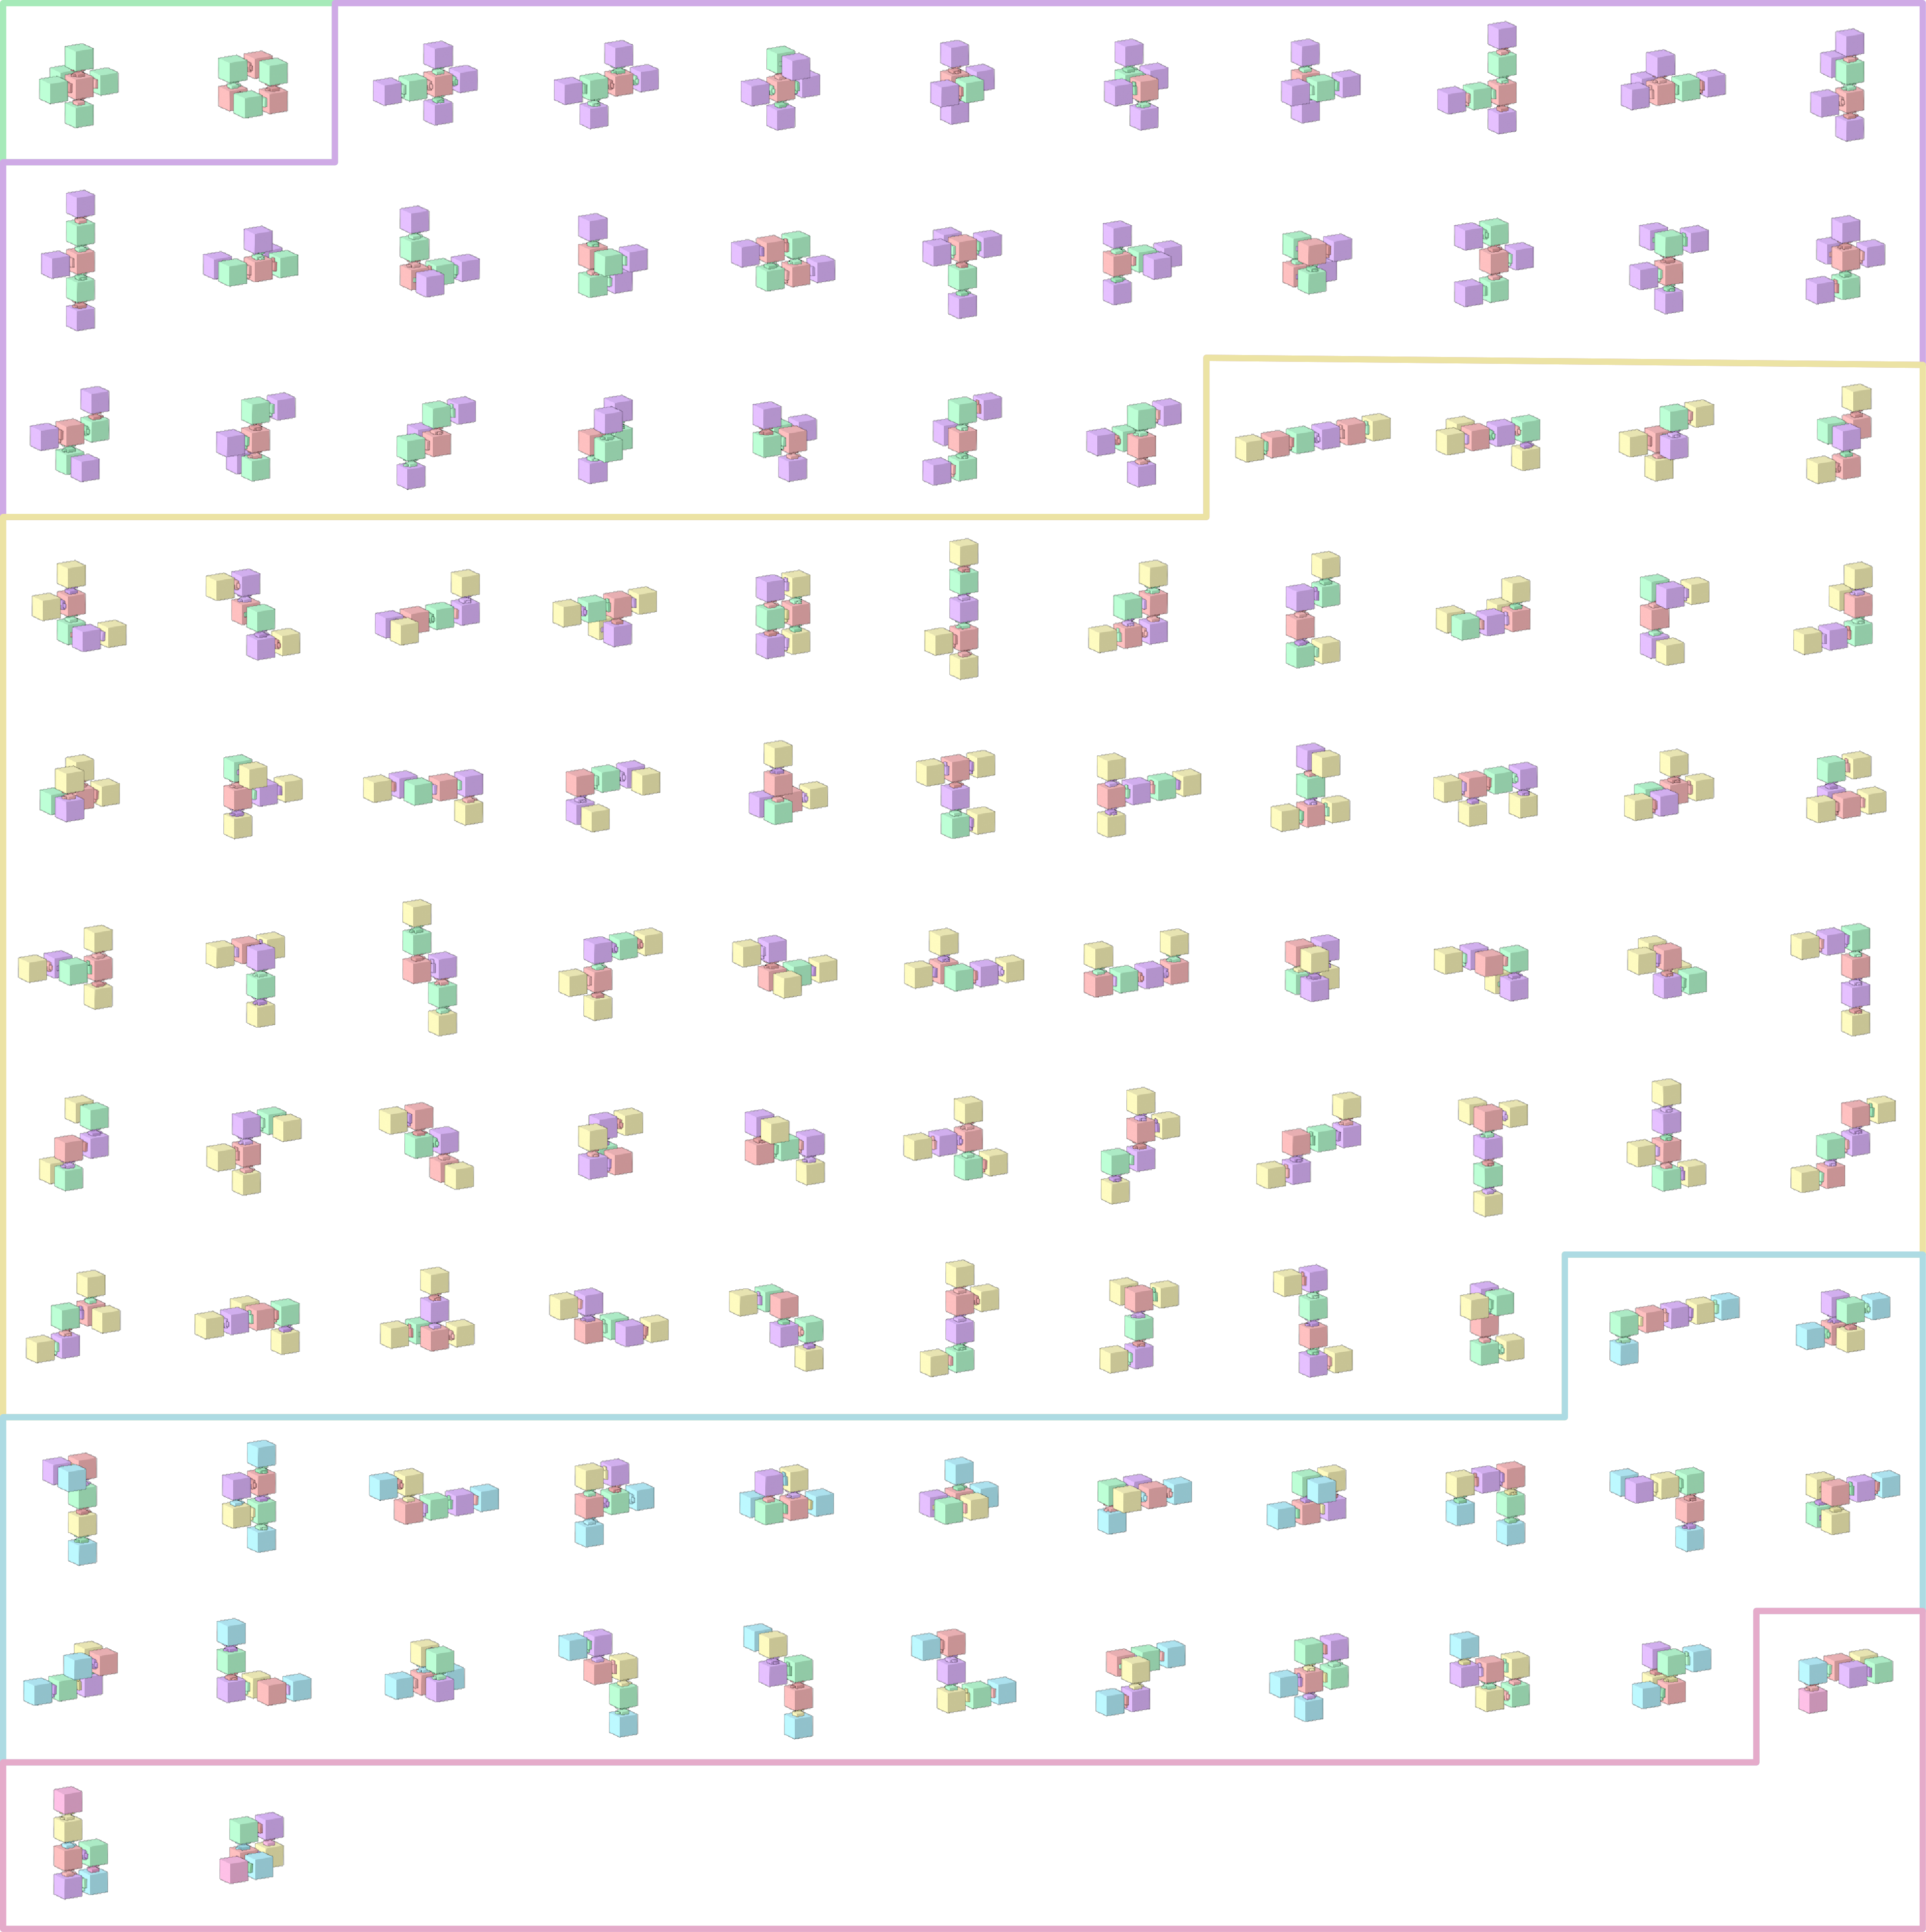
\includegraphics[width=\textwidth,]{figures/6-mers/6-mers.png}
    \caption{All 112 free 6--mer polycubes (3D) grouped by their smallest solved complexity (\(\widetilde{K}_s\)). The polyominoes are ordered from left to right, top to bottom, primarily according to the minimal number of species (\(\widetilde{K}_s\)), secondarly the number of colours (\(\widetilde{K}_c\)) needed for their assembly. Lines are drawn to group the polyominoes with equal \(\widetilde{K}_s\), showing that there are 
    2 polycubes with \(\widetilde{K}_s=2\),
    27 polycubes with \(\widetilde{K}_s=3\),
    57 polycubes with \(\widetilde{K}_s=4\),
    23 polycubes with \(\widetilde{K}_s=5\), and
    3 polycubes with \(\widetilde{K}_s=6\)
    }
    \label{fig:6-mers_grid}
\end{figure}

Figure~\ref{fig:6-mer_distribution} also highlights another limitation with the sampled results; the number of 6-mer polycubes found, 166, is larger than the unique number of possible 6-mer polycubes (112). Likely, this is due to some rules, despite extensive testing, not being fully deterministic, thereby creating redundant polycube groups during the sampling. Since the polycube count is still within the correct order of magnitudes (Figure~\ref{fig:main_distr}), adressing this discrepancy is deemed out of scope for this work.


\begin{figure}[h]
    \centering
    \begin{overpic}[width=\textwidth]{figures/6-mers/distribution.eps}
        \put(30, 330){\makebox(0,0){\rotatebox{90}{Number of colours (\(\widetilde{K}_c\))}}}
        \put(210, 10){Number of species (\(\widetilde{K}_s\))}

        \put(30, 710){\makebox(0,0){\rotatebox{90}{Count}}}
        \put(690, 0){Count}
        \put(890, 720){SAT solver}
        \put(890, 690){\(I_{5_s,31_c}^{3D}\)}
        \put(850, 780){Dataset}
        \put(850, 650){Count}
    \end{overpic}
    \caption{Complexity distributions for 6--mer polycubes. The blue distribution (left) corresponds to the minimal SAT solver solutions to all 112 possible 3D 6--mers. The orange distribution (right) corresponds to the 6--mers found through randomly sampling the \(I_{5_s,31_c}^{3D}\) space of polycube rules.}
    \label{fig:6-mer_distribution}
\end{figure}


% Ard: Compare ch4 back to previous results. Make grids from random samples, colour by frequency.

% 1) Take a high probability structure (e.g. the cube) and see how often different rules are found by random sampling  --- is it roughly true that P(ruleset) ~ 2^(size)  -- log P(ruleset) ~ size of ruleset

% 2) I would do this for some of the say 16mers or other 2D structures e.g. in the paper with Iain -- we simply found the K by looking at the shortest code found by sampling. Question" how good is this in practice. --  you did this as well in your plots.


\FloatBarrier
\section{Assembly in a continuous model}
While the stochastic assembler works well to test determinism, it does not have realistic assembly dynamics. To study how the rule affects assembly dynamics, we now turn to a more sophisticated patchy particle simulation.

\subsection{Patchy particle simulation}
\label{sec:patchy_particles}

% Andrew: Describe! Diffusion, in position and orientation. Hence need to constrain interactions tightly to ensure good mapping to more abstract models.

Besides discrete tile models, self--assembly can also be modelled using simulations of rigid--body spheres called \emph{patchy particles}. The particles move using Molecular Dynamics (MD), updating their positions and orientations according to Newtown's laws of motion. An Andersen--like thermostat~\cite{russo2009reversible} is used to manage the energy in the system (there is no explicit solvent) and to keep a constant, specified temperature. Furthermore, each particle has one or more patches that can interact with and bind the patches of other particles. The angles at which two patches interact can be modulated to allow for wider or more narrow patches, allowing us to study how the bond flexibility affects the assembly dynamics. Further details of the patchy particle model are provided in Appendix~\ref{ch:appendix_patchy}.

As seen in Figure~\ref{fig:patchy_particles}, the patchy particle simulator included in the oxDNA package \cite{rovigatti2015comparison} has previously been used by Romano et al.\, to verify the patchy interactions designed by their SAT--solver method \cite{romano2020designing}. A derivative of that patchy particle model is used here, modified to include torsional interactions to account for the polycube requirement of patch orientation alignment.

\begin{figure}[h]
  \centering
  \vspace{1em}
  \begin{overpic}[width=\textwidth]{figures/patchy_particles.png}
    \put(0,310){a)}
    \put(280,310){b)}
    \put(650,310){c)}
  \end{overpic}
  \caption{Patchy particle simulation, adapted from \cite{romano2020designing}. \textbf{a)} The unit cell of a tetrastack lattice build with patchy particles. \textbf{b)} Simulation snapshot of a forming tetrastack lattice. Note the free--flowing particles that have not yet attached the growing latttice they surround. \textbf{c)} Tetrastack particle energy plotted over simulation time for different temperatures. Sudden drops in energy correspond to nucleation events (where the lattices start forming).}
  \label{fig:patchy_particles}
\end{figure}

\subsection{Yield calculation}

The patchy particle simulation yields are mainly calculated using edge-induced subgraph isomorphism \cite{networkx}. 
We annotate \(\sigma(G_a,G_b) == \text{True}\) if the graph \(G_a\) is an edge-induced subgraph of the graph \(G_b\).
The connectivity graph \(G_i\) for each assembled particle cluster is compared to the graph for the intended shape \(G_{correct}\). If \(G_i\) is a large enough edge-induced subgraph of \(G_{\text{correct}}\), meaning that its particles are connected like a large enough subset (the current results use a 75\% size cutoff) of the correct shape, it contributes to the yield with its fraction of correctly assembled particles:
\begin{equation}
    Y_{c} = \sum_{G_i \in c} \begin{cases} 
           \frac{\left|N(G_i)\right|}{\left|N(G_{\text{correct}})\right|} & \text{if } \sigma(G_i,G_{\text{correct}}) \\
                          0 & \text{otherwise}
                        \end{cases}
\end{equation}

The subgraph calculation becomes very compute-intensive for larger and more highly connected graphs, so for the \(4 \times 4 \times 4\) solid cube we instead check the cluster's species composition, making sure that its species are a subset (with duplicates) of the intended shape. For the minimal solution, this underestimates the yield for some temperatures compared to the subgraph measure, as the solution can produce correct shapes with varying species compositions (but some mismatched connections). 

The other exception is used in the case of the werewolf design (Section~\ref{sec:multifarious}), where the connectivity graph of the human structure is a subgraph of the connectivity graph of the wolf structure. To tell the two shapes apart, we check both the connectivity graph and the species composition.


\subsection{Simulation results}

Next, we simulate and compare the assemblies of the fully addressable and minimal solutions to the shapes introduced in Section~\ref{sec:example_solves}. Figure~\ref{fig:shapeKinetics} shows the assembly yields for three different shapes, using either their minimal or their fully addressable solutions. At low-enough temperatures, all solutions assemble with good yields. As can be seen, the minimal solutions perform just as well as the fully addressable. This is not very significant for the Letter J shape since the complexity difference is small (Figure~\ref{fig:letter_J}). However, for the robot and swan, having similar assembly kinetics using 8 unique species instead of 17 (for the robot, Figure~\ref{fig:robot}), or even 5 instead of 9 (for the swan, Figure~\ref{fig:swan}) can provide considerable experimental resource savings.


\begin{figure}[h]
    \centering
    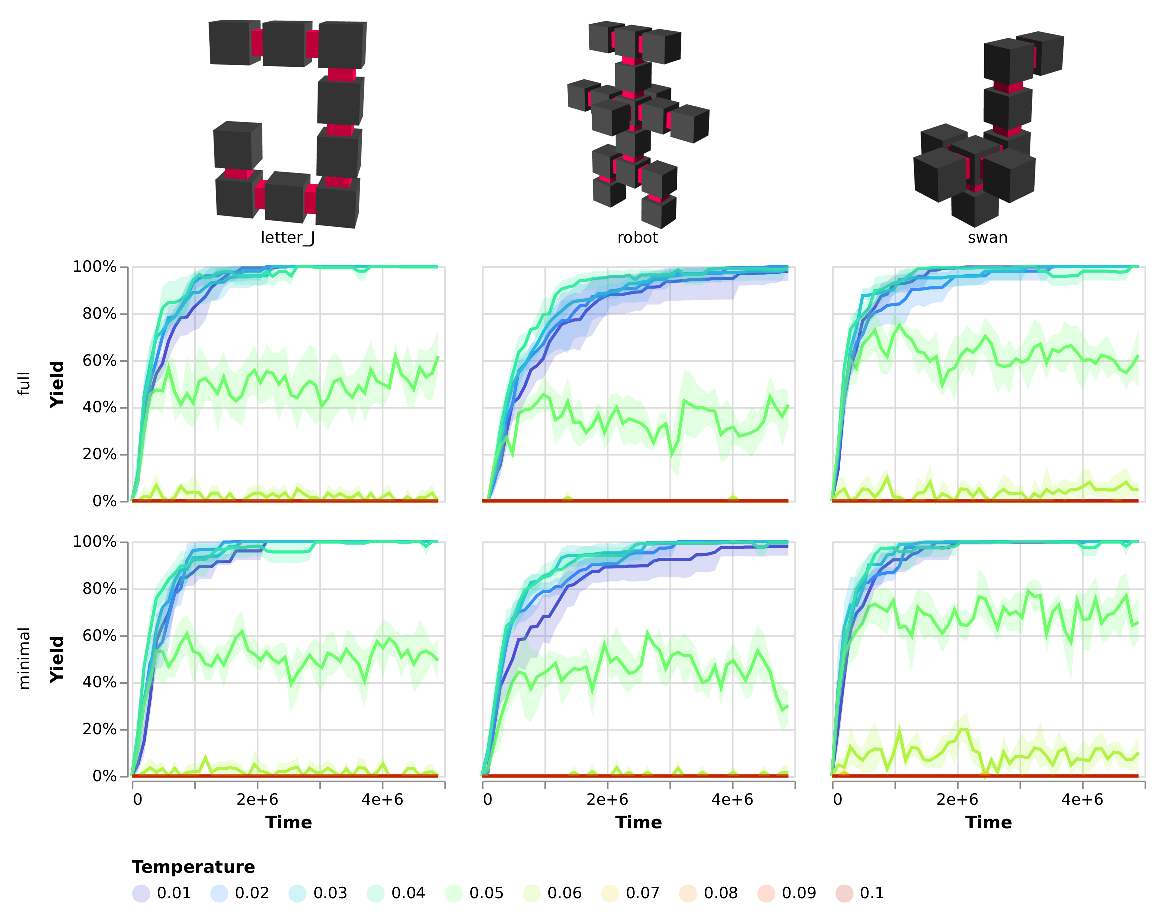
\includegraphics[width=\linewidth]{figures/patchysim/shapeKinetics.eps}
    \caption{Assembly kinetics for three shapes. The top row column shows the fully addressable solution while the bottom shows the minimal solution. Solid lines are mean values from 5 duplicate simulations, error bands show the 95\% confidence interval band. Each simulation is done using the narrow type \(0\) potential (patch width = \(2.346\)) at a \(0.1\) particle density. Temperature and time is measured in simulation units.}
    \label{fig:shapeKinetics}
\end{figure}

Figure~\ref{fig:cubePotentials} shows the yield plots for three different solutions for assembling the hollow \(3 \times 3 \times 3\) cube from Figure~\ref{fig:hollow_cube}; the fully addressable solution with 20 species, a significantly smaller solution using four species, and the minimal solution with only two species. We also investigate the effects of bond flexibility by simulating the assemblies at different patch interaction widths (defined in Figure~\ref{fig:pp}). More narrow patch widths (less flexible bonds) lead to slower assembly times, which can be expected since particles are less likely to bind. On the other hand, bonds that are too flexible can cause unwanted bonding and aggregation.

While the previous three shapes are unlikely to assemble into anything other than the intended size, the cubes can aggregate into clusters many times larger than intended if their bonds are flexible enough. This happens because cubes are self--limiting through their geometry, which works less well on flexible patchy particles compared to the rigid lattice of the stochastic assembler. In contrast, the previous shapes are self--limiting through their topology, with no loops in their connectivity graphs, so while flexible bonds can lead to deformations, their topology will remain the same. For patches without torsion, only the fully addressable solution manages to assemble with a good yield. More distinct species create larger connectivity graph loops, with a mitigating effect on aggregation with the cost of a longer assembly time. 

The minimal solution, however, performs very well for the intermediate patch widths \(0.955\) and \(0.657\), assembling fast and at a high yield. These results show that not only can the minimised assembly sets provide resource savings, but they can also lead to faster assembly dynamics and better yields. For these designs, the patches are narrow enough to avoid aggregation, while the low species count improves the assembly speed by being more available (with one in two being better odds than one in 20). We expect the even smaller patch widths to achieve a high yield as well, eventually.

\begin{figure*}[h]
    \centering
    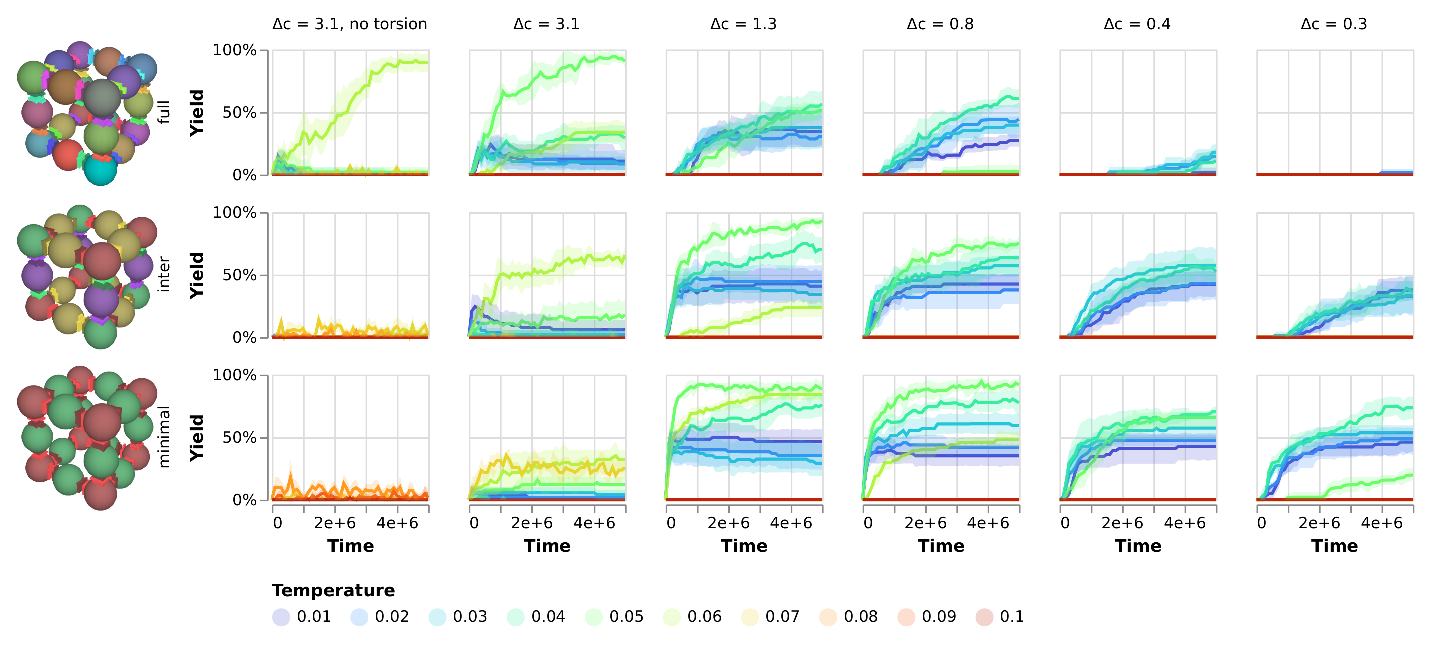
\includegraphics[width=\linewidth]{figures/patchysim/cubePotentials.eps}
    \caption{Assembly yield for hollow \(3 \times 3 \times 3\) cube designs. The top row shows the \href{https://akodiat.github.io/polycubes/?assemblyMode=stochastic&rule=00040109020c000089110200001491010218000001018e1c002001259e000000a5290200002ca901b200000001019a30963401010200863801010200ba00013d02400000bd450200b600c5010248ae4c01010200ce00e101d20000000101ca5000000101c254de000159d600a25c010102000000d9610200}{fully addressable solution}, using 20 species and 24 colours. The middle row shows an \href{https://akodiat.github.io/polycubes/?assemblyMode=stochastic&rule=90000800000600040090000d000000008b8d000011860000}{intermediate solution}, using 4 species and 4 colours. The bottom row shows the \href{https://akodiat.github.io/polycubes/?assemblyMode=stochastic&rule=070000070500868700000000}{minimal solution}, using 2 species and 1 colour. Columns correspond to different interaction potentials, with the leftmost column showing wide patches without torsion. The remaining columns show torsional patches with decreasing patch width. Solid lines are mean values from 5 duplicate simulations, and error bands show the 95\% confidence interval band. Each simulation has a \(0.1\) particle density.}
    \label{fig:cubePotentials}
\end{figure*}

Figure~\ref{fig:solidCubePotentials} shows yield plots for the solid \(3 \times 3 \times 3\) cube from Figure~\ref{fig:solid_cube}. The fully addressable solution here requires 27 species, the intermediate uses six, and the minimal solution only four.  The trends seen in Figure~\ref{fig:cubePotentials} can be seen here as well, with the exception that the wider, more flexible patches now perform much better. Here the aggregation is mitigated by the cubes being more interconnected. While, without torsion, a single bond could rotate freely around its axis, the particles are held in place by multiple bonds along orthogonal axes, binding more strongly the more bonds they form.

\begin{figure*}[h]
    \centering
    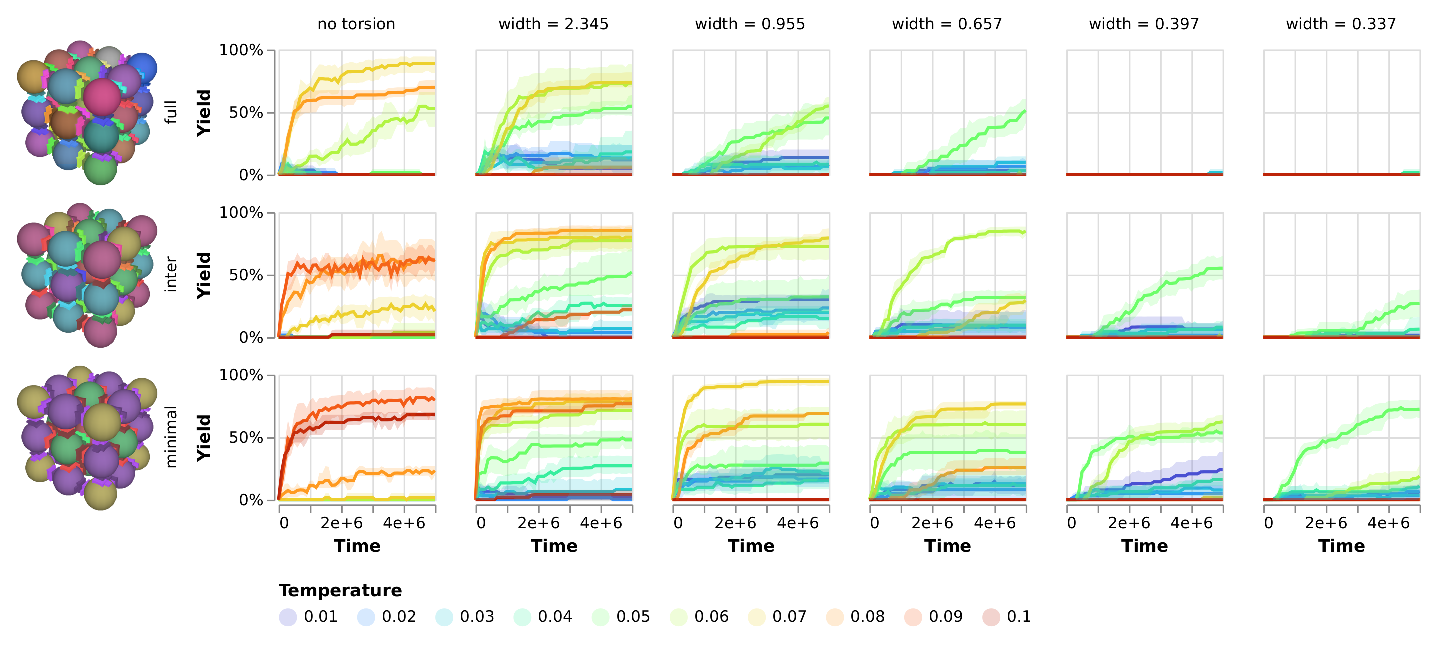
\includegraphics[width=\linewidth]{figures/patchysim/solidCubePotentials.eps}
    \caption{Assembly yield for solid \(3 \times 3 \times 3\) cube designs. The top row shows the \href{https://akodiat.github.io/polycubes/?decRule=|1:0||2:1||3:0_-1:2|4:0||5:1||6:0_|7:0|-2:1|8:1||9:0_|10:0||11:1|-3:2|12:0_-4:2|||13:1||14:0_-7:2|15:0|-5:1|16:1||17:0_-10:2|18:0||19:1|-6:2|20:0_-15:2||-13:1|21:1||22:0_-18:2|||23:1|-14:2|24:0_|25:0|-11:1|26:1|-9:2|27:0_|28:0||29:1|-12:2|_-25:2|30:0|-19:1|31:1|-17:2|32:0_-28:2|33:0||34:1|-20:2|_-30:2||-23:1|35:1|-22:2|36:0_-33:2|||37:1|-24:2|_|38:0|-29:1|39:1|-27:2|_-38:2|40:0|-34:1|41:1|-32:2|_-40:2||-37:1|42:1|-36:2|_|43:0|-8:1|||44:0_-43:2|45:0|-16:1|||46:0_-45:2||-21:1|||47:0_|48:0|-26:1||-44:2|49:0_-48:2|50:0|-31:1||-46:2|51:0_-50:2||-35:1||-47:2|52:0_|53:0|-39:1||-49:2|_-53:2|54:0|-41:1||-51:2|_-54:2||-42:1||-52:2|}{fully addressable solution}, using 27 species and 54 colours. The middle row shows an \href{https://akodiat.github.io/polycubes/?assemblyMode=stochastic&rule=10101113232391001d1d8c2400a2949495970c00a5001b1a1700009d0a8598008a000400}{intermediate solution}, using 6 species and 9 colours. The bottom row shows the \href{https://akodiat.github.io/polycubes/?assemblyMode=stochastic&rule=0a0a0b0a0908878784868b00060000078e8f000c0c00000e}{minimal solution}, using 4 species and 3 colours. Columns correspond to different interaction potentials, with the leftmost column showing wide patches without torsion. The remaining columns show torsional patches with decreasing patch width. Solid lines are mean values from 5 duplicate simulations, and error bands show the 95\% confidence interval band. Each simulation has a \(0.1\) particle density.}
    \label{fig:solidCubePotentials}
\end{figure*}

Finally, Figure~\ref{fig:cube4_potentials} shows the yield plots for the solid \(4 \times 4 \times 4\) cube from Figure~\ref{fig:cube4}, for the fully addressable solution with 64 species and the minimal solution with only six species.

\begin{figure}[h]
    \centering\includesvg[width=\textwidth, inkscapelatex=false]{figures/patchysim/cube4.svg}
    \caption{Assembly yield %at \(t=5\times 10^7\) 
    for two solid \(4 \times 4 \times 4\) cube designs. The top row shows the \href{https://akodiat.github.io/polycubes/?decRule=|-3:2||-7:1|1:2|2:0_3:0|4:0||-23:1|5:2|6:0_|-21:2|7:1|8:1|9:2|10:0_|-27:2||-41:1||-1:0_|-12:2||-15:1|-2:2|11:0_12:0|13:0||-33:1|-6:2|14:0_|-31:2|15:1|16:1|-10:2|17:0_|-36:2||-59:1|-11:2|_-4:2|18:0||-44:1|19:2|20:0_21:0|22:0|23:1|24:1|25:2|26:0_27:0|28:0||-55:1||-5:0_-13:2|29:0||-62:1|-20:2|30:0_31:0|32:0|33:1|34:1|-26:2|35:0_36:0|37:0||-71:1|-14:2|_|-48:2|-8:1|38:1|39:2|40:0_|-53:2|41:1|42:1||-9:0_-22:2|43:0|44:1|45:1|46:2|47:0_48:0|49:0|-24:1|50:1|51:2|52:0_53:0|54:0|55:1|56:1||-25:0_|-65:2|-16:1|57:1|-40:2|58:0_|-69:2|59:1|60:1|-17:2|_-32:2|61:0|62:1|63:1|-47:2|64:0_65:0|66:0|-34:1|67:1|-52:2|68:0_69:0|70:0|71:1|72:1|-35:2|_-18:2|||-81:1|73:2|74:0_-28:2|75:0||-90:1||-19:0_-29:2|||-92:1|-74:2|76:0_-37:2|77:0||-79:1|-30:2|_-77:2|||-102:1|-76:2|_-70:2|78:0|79:1|80:1|-64:2|_-43:2||81:1|82:1|83:2|84:0_-49:2|85:0|-45:1|86:1|87:2|88:0_-54:2|89:0|90:1|91:1||-46:0_-61:2||92:1|93:1|-84:2|94:0_-66:2|95:0|-63:1|96:1|-88:2|97:0_98:0|99:0|-72:1|100:1|-68:2|_|-98:2|-60:1|101:1|-58:2|_-78:2||102:1|103:1|-94:2|_-99:2|104:0|-80:1|105:1|-97:2|_|-109:2|-38:1||106:2|107:0_|-113:2|-42:1|108:1||-39:0_109:0|110:0|-50:1||111:2|112:0_113:0|114:0|-56:1|115:1||-51:0_-85:2||-82:1|116:1|117:2|118:0_-110:2|119:0|-86:1||120:2|121:0_-114:2|122:0|-91:1|123:1||-87:0_|-125:2|-57:1||-107:2|124:0_125:0|126:0|-67:1||-112:2|127:0_-95:2||-93:1|128:1|-118:2|129:0_-126:2|130:0|-96:1||-121:2|131:0_|-132:2|-101:1||-124:2|_132:0|133:0|-100:1||-127:2|_-104:2||-103:1|134:1|-129:2|_-133:2|135:0|-105:1||-131:2|_-75:2|||-137:1||-73:0_-135:2||-134:1||-136:2|_-130:2||-128:1||-140:2|136:0_-89:2||137:1|138:1||-83:0_-119:2||-116:1||139:2|140:0_-122:2||-138:1|141:1||-117:0_|-142:2|-108:1|||-106:0_142:0|143:0|-115:1|||-111:0_-143:2|144:0|-123:1|||-120:0_-144:2||-141:1|||-139:0}{fully addressable solution}, using 64 species and 144 colours. The bottom row shows the \href{https://akodiat.github.io/polycubes/?decRule=-1:2|-4:1|1:1|-4:1|-8:1|-4:1_-3:2|-4:2|-4:2|8:1|3:1|-4:0_9:1|7:3|4:1||-9:2|-5:0_6:3|2:1|5:1|||-7:2_-7:0||-6:0|2:3||5:1_|-2:1||-2:1||-2:1}{minimal solution}, using 6 species and 8 colours. Columns correspond to different interaction potentials, with the leftmost column showing wide patches without torsion. The remaining columns show torsional patches with decreasing patch width. Each simulation has a \(0.1\) particle density.}
    \label{fig:cube4_potentials}
\end{figure}

\FloatBarrier
\section{DNA origami implementation}
To demonstrate a possible experimental realisation of the six-valent cubic-shaped designs considered here, Dr. Michael Matthies assisted by designing a wireframe DNA origami cube using ATHENA \cite{athena}, and the oxView software tools \cite{poppleton2020design, bohlin2022oxview}. A complete DNA polycube design can be automatically generated by replacing the abstract cubes of the stochastic assembly result with connected origami structures,

A DNA wireframe \(3 \times 3 \times 3\) cube design was verified with oxDNA \cite{vsulc2012sequence,Snodin2015,ouldridge2011structural} simulation. The DNA origami cubes can bind to each other through single-stranded (ssDNA) overhangs. One ``patch'' of our abstract polycube model corresponds to a set of ssDNA overhangs, each with a unique sequence, placed on the edges of a cube face, thus realising a patch with a well-defined orientation. Complementary patches are provided with complementary overhangs. Figure~\ref{fig:hollowCubeDNA} shows the structure, and structural fluctuations, of a minimal wireframe $3\times3\times3$ cube assembly, realised using the origami design, as represented in an oxDNA simulation.

\begin{figure}[h]
    \centering
    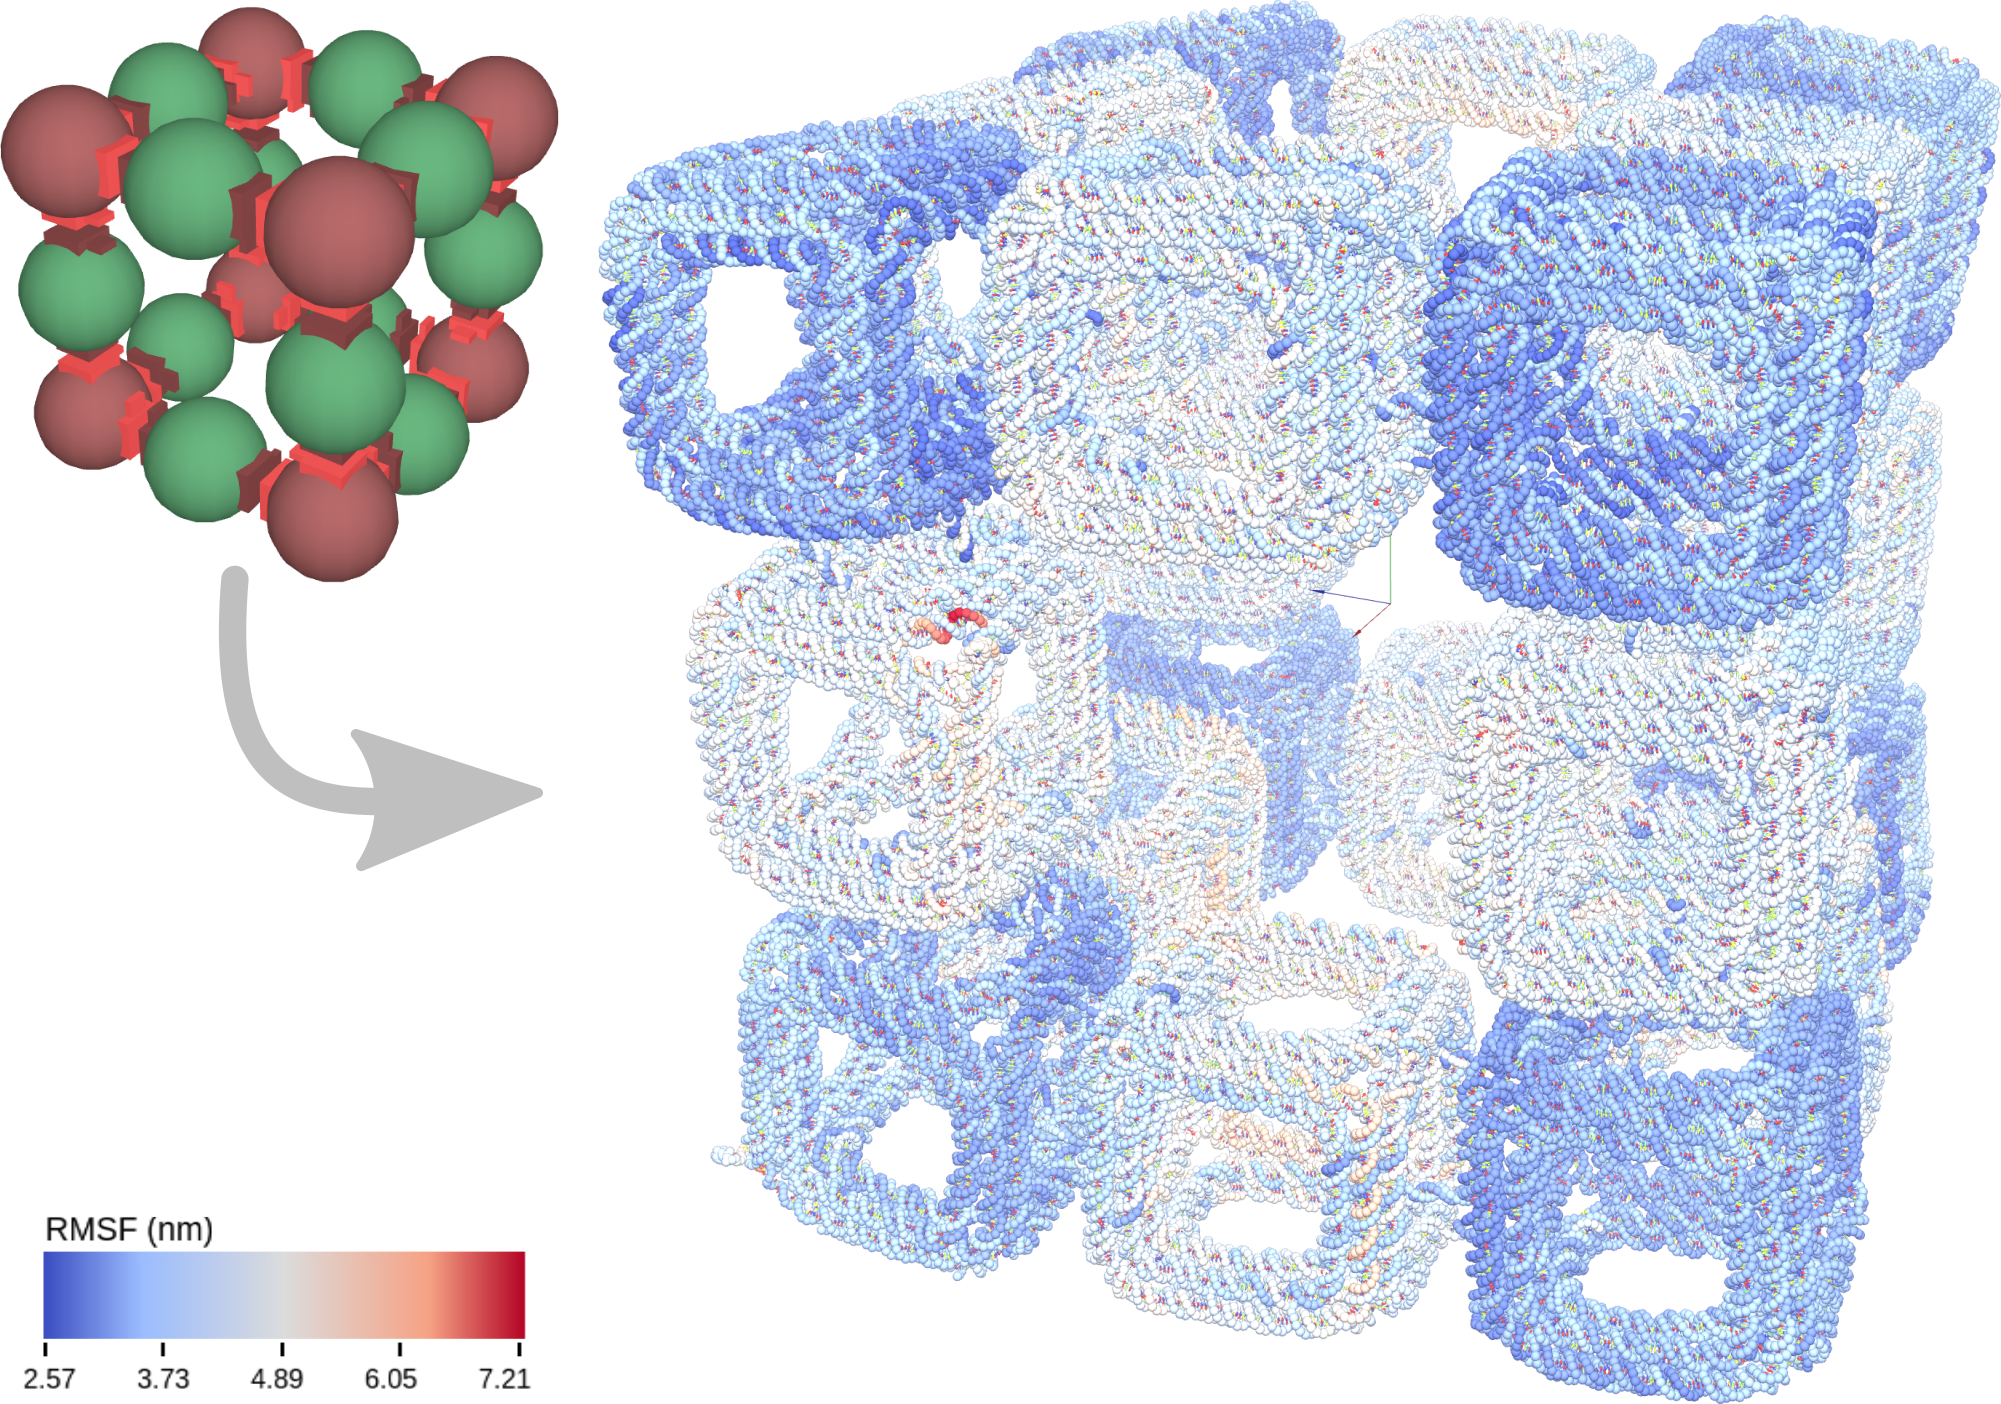
\includegraphics[width=\linewidth]{figures/DNA_polycube.png}
    \caption{Mean structure and root-mean-square-fluctuation (RMSF) analysis (right) of the wireframe \(3 \times 3 \times 3\) cube \href{https://akodiat.github.io/polycubes/?assemblyMode=stochastic&rule=070000070500868700000000}{minimal solution} (top left), formed from DNA origami ``patchy'' particles and simulated using oxDNA for a duration corresponding to about $10^{-3}$~s.
    }
    \label{fig:hollowCubeDNA}
\end{figure}


\FloatBarrier
\section{Multifarious assemblies}
\label{sec:multifarious}

Another feature of the SAT solver approach is the ability to design \emph{multifarious} assemblies, that is, rules that can assemble into more than one shape. This is done by defining multiple distinct shapes next to each other as input to the solver. As an example of this, we solve a ``wolf'' and a ``human'' shape first separately (Figure~\ref{fig:werewolf}.a--b), then as a single ``werewolf'' shape specification (Figure~\ref{fig:werewolf}.c).

The wolf shape consists of 14 cubes, while the human has 13, so they are roughly the same size. While the fully addressable multifarious solution (``werewolf'') would require 27 species, the SAT solver approach found a minimal solution using only ten species and eight colours, with two species shared between both shapes.

We assemble the three minimal solutions (human, werewolf, and wolf) and compare the yields at which they assemble either human or wolf shapes. As seen in Figure~\ref{fig:multifarious_sim} the individual human and wolf shapes assemble with 100\% yield (at sufficiently low temperatures), while the werewolf design assembles with approximately 50\% yield for either shape, with the wolf being favoured slightly at lower temperatures. The relative concentration of species in the werewolf simulations was chosen so that there was sufficient material to assemble either ten humans or ten wolves. Any chimeric clusters, with part human and part wolf, are not possible as such solutions have been ruled out by the stochastic assembler.


\begin{figure}
    \centering
    \begin{overpic}[width=\textwidth]{figures/solve/werewolf.eps}
        \put(10,850){a)}
        \put(10,330){b)}
        \put(380,570){c)}

        \put(-10, 710){\makebox(0,0){\rotatebox{90}{Number of colours (\(\widetilde{K}_c\))}}}
        \put(30, 530){Number of species (\(\widetilde{K}_s\))}

        \put(-10, 160){\makebox(0,0){\rotatebox{90}{Number of colours (\(\widetilde{K}_c\))}}}
        \put(30, -10){Number of species (\(\widetilde{K}_s\))}

        \put(350, 300){\makebox(0,0){\rotatebox{90}{Number of colours (\(\widetilde{K}_c\))}}}
        \put(520, -10){Number of species (\(\widetilde{K}_s\))}
    \end{overpic}
    \caption{Designing a multifarious ``werewolf'' shape. \textbf{a)} Solution landscape and depiction of the individual ``wolf'' shape \textbf{b)} Solution landscape and depiction of the individual ``human'' shape. \textbf{c)} Solution landscape and depiction of the combined ``werewolf'' shape. The coordinates of both shapes are added as input to the SAT solver, thus producing solutions that can assemble both shapes.}
    \label{fig:werewolf}
\end{figure}

\begin{figure}
    \centering
    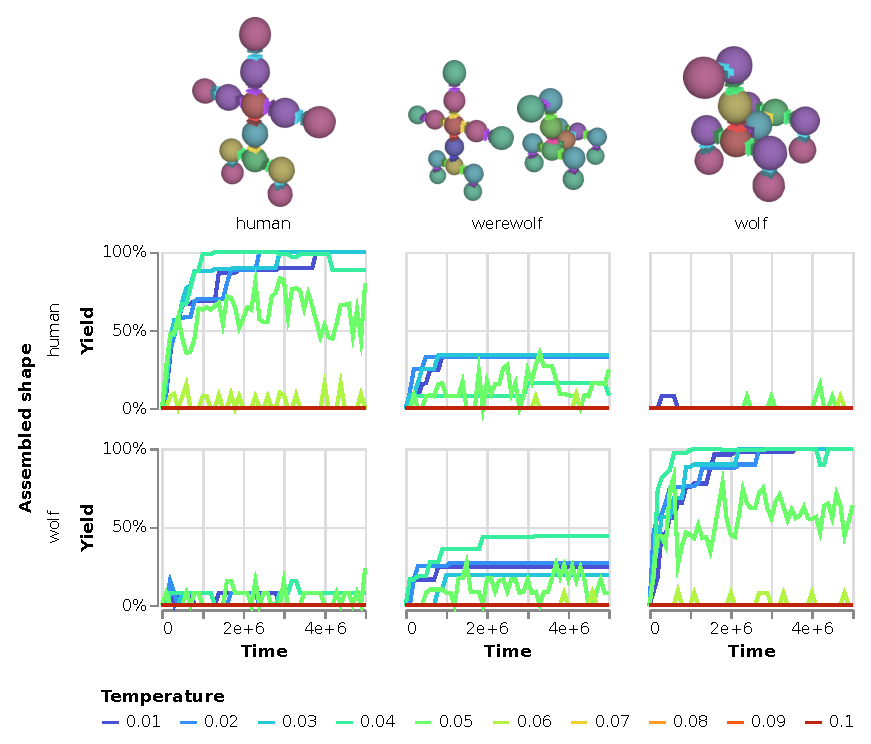
\includegraphics[width=\linewidth]{figures/patchysim/werewolf.eps}
    \caption{Multifarious werewolf assembly. The leftmost column shows the minimum solution for the  \href{https://akodiat.github.io/polycubes/?assemblyMode=stochastic&rule=00000e040f0c88880000120000008f1600000000000b1400938700000000000000000096}{``human''} shape, the rightmost shows the minimum solution for the  \href{https://akodiat.github.io/polycubes/?assemblyMode=stochastic&rule=04000909000c0013000009098a00001400000000000009840000938c0000000000009700}{``wolf''} shape, and the middle column shows the minimum solution that can reliably assemble both human and wolf shapes, here labelled \href{https://akodiat.github.io/polycubes/?assemblyMode=stochastic&rule=11051013000018001d1d0008001700001d1da1001d1d00009e00000c0000000000000d93000000001d98000000002284000097880000000000008f00}{``werewolf''}. The top and bottom rows show the yield at which the designs assemble the ``human'' and the ``wolf'' shapes respectively. Each simulation is done using the wide torsional patch potential with width = \(2.346\)) at a \(0.1\) particle density.}
    \label{fig:multifarious_sim}
\end{figure}

\FloatBarrier
\section{Conclusion}
While Chapter~\ref{ch:polycubes1} showed how to map input rules into output shapes, this chapter has shown how to find the input rules that assemble a given shape, making it possible to determine the minimal complexity rule for an intended design (including multifarious designs). As was seen in Chapter~\ref{ch:polycubes_intro}, many current experimental works either use unique nanoparticles for each position in a final assembly or reuse particles in periodic or otherwise simple structures. The systematic design pipeline presented here should facilitate the design of bounded structures, saving resources and minimising cross-talk between interfaces.

The design pipeline shown here can explore the landscape of assembly solutions for arbitrary shapes. In many cases, the minimum solution comprises significantly fewer particles than the target structure and assembles more rapidly than the solution in which every component is unique, with comparable or higher yields. 

For highly specific binding domains (such as those relevant for protein assembly), the minimal solution assembles better than more complex designs. This result suggests an interesting evolutionary hypothesis:  The recently discovered non-adaptive bias towards minimal protein complex designs~\cite{johnston2021} may produce complexes that will assemble better, providing an additional adaptive evolutionary driver towards simpler and therefore more symmetric structures.

Similarly, these results indicate that not only does a minimum assembly design presents an advantage in terms of manufacturing costs for certain experimental realisations and conditions, but it is also predicted to better assemble than the fully addressable option. Generally, the kinetics of assembly is slower for narrower patch interactions, as random collisions are less likely to lead to successful bond formation. Additionally, two randomly chosen particles are less likely to have compatible interfaces for the fully addressable system. Hence, the structure growth is expected to be slower than for the minimal solution.

These results are likely to benefit the DNA nanotechnology field: the requirement for fewer unique components would mean significant savings in both time and resources, and we have developed a new automated design tool that can convert target structure design to a nucleotide-level coarse-grained DNA nanostructure representation for computational verification or for guiding an experimental design. Finally, the inverse design method is also applicable to other designed self-assembling systems, such as multi-component protein structures or coated nanoparticles \cite{zhu2021protein,xiong2020three}.